\chapter{Market analysis}\label{ch:market}
\section{Introduction}\label{sec:market:introduction}
The global market for educational application for children is extremely challenging. With nearly \$400 million of revenue in the year 2017 and estimated \$1 billion in 2022 \cite{christianaWhatSizeKids2017} (which equals to around 22\% Compound Annual Growth Rate) it is one of the fastest-growing categories. Hence, it is almost impossible to analyze every available application. Section \ref{sec:market:solutions}, however, will sum up advantages and disadvantages of a few examples of possible direct competition. Section \ref{sec:market:conclusions} will summarize and conclude the analysis.


\section{Overview of existign solutions}\label{sec:market:solutions}
All of the gathered information is based on official Google Play (Apple App Store if not available) documentation and, if possible, physical installation of an app. Devices used to test applications were Samsung Galaxy A50 (Android, version 10) and Apple iPad Pro 2020 (iOS, version 14.2). Screenshots are taken on an emulated LG Nexus 5X (Android, version 10) or mentioned iPad.


\subsection{iRewardChart}\label{subsec:market:solutions:irewardchart}
Application \textit{iRewardChart} \cite{IRewardChartAppsGoogle,IRewardChartChoreTracker}, originally released in 2009, was one of the first on the market. It is available both on Android and iOS platform. Its target group are children aged three and older. It has more than 10000 downloads on Google Play, but its average rating is 2.7 (on a scale from 1 to 5). Application's size is 7MB. It can be run on a device with Android 4.1 and higher. Its last update was in October 2017, and the project website\footnote{www.irewardchart.com} is not reachable, which suggest it not being supported anymore.
\\\\
\textit{isRewardChard} is rather simple to use, yet its design is outdated. Its main screen is a week table view with particular tasks represented as stars. Tasks can be marked with multiple yellow (positive) and red (negative) stars, which can be redeemed for rewards. The software has a feeble user experience (including occasional errors presented to the user) and gives an impression of an expense tracker more than a family application. It allows for tasks and rewards customization, as well as multiple children management, though only in the paid version. It lacks a child's perspective as well.
\\\\
Example screenshots of the \textit{iRewardChart} application were presented in Figure~\ref{fig:applications:irewardchart}. A summary of its positives and negatives was presented in Table~\ref{tab:applications:irewardchart}.
\\
\begin{figure}
\centering
\begin{tabular}{cc}
\subcaptionbox{Calendar view (main screen)}{ 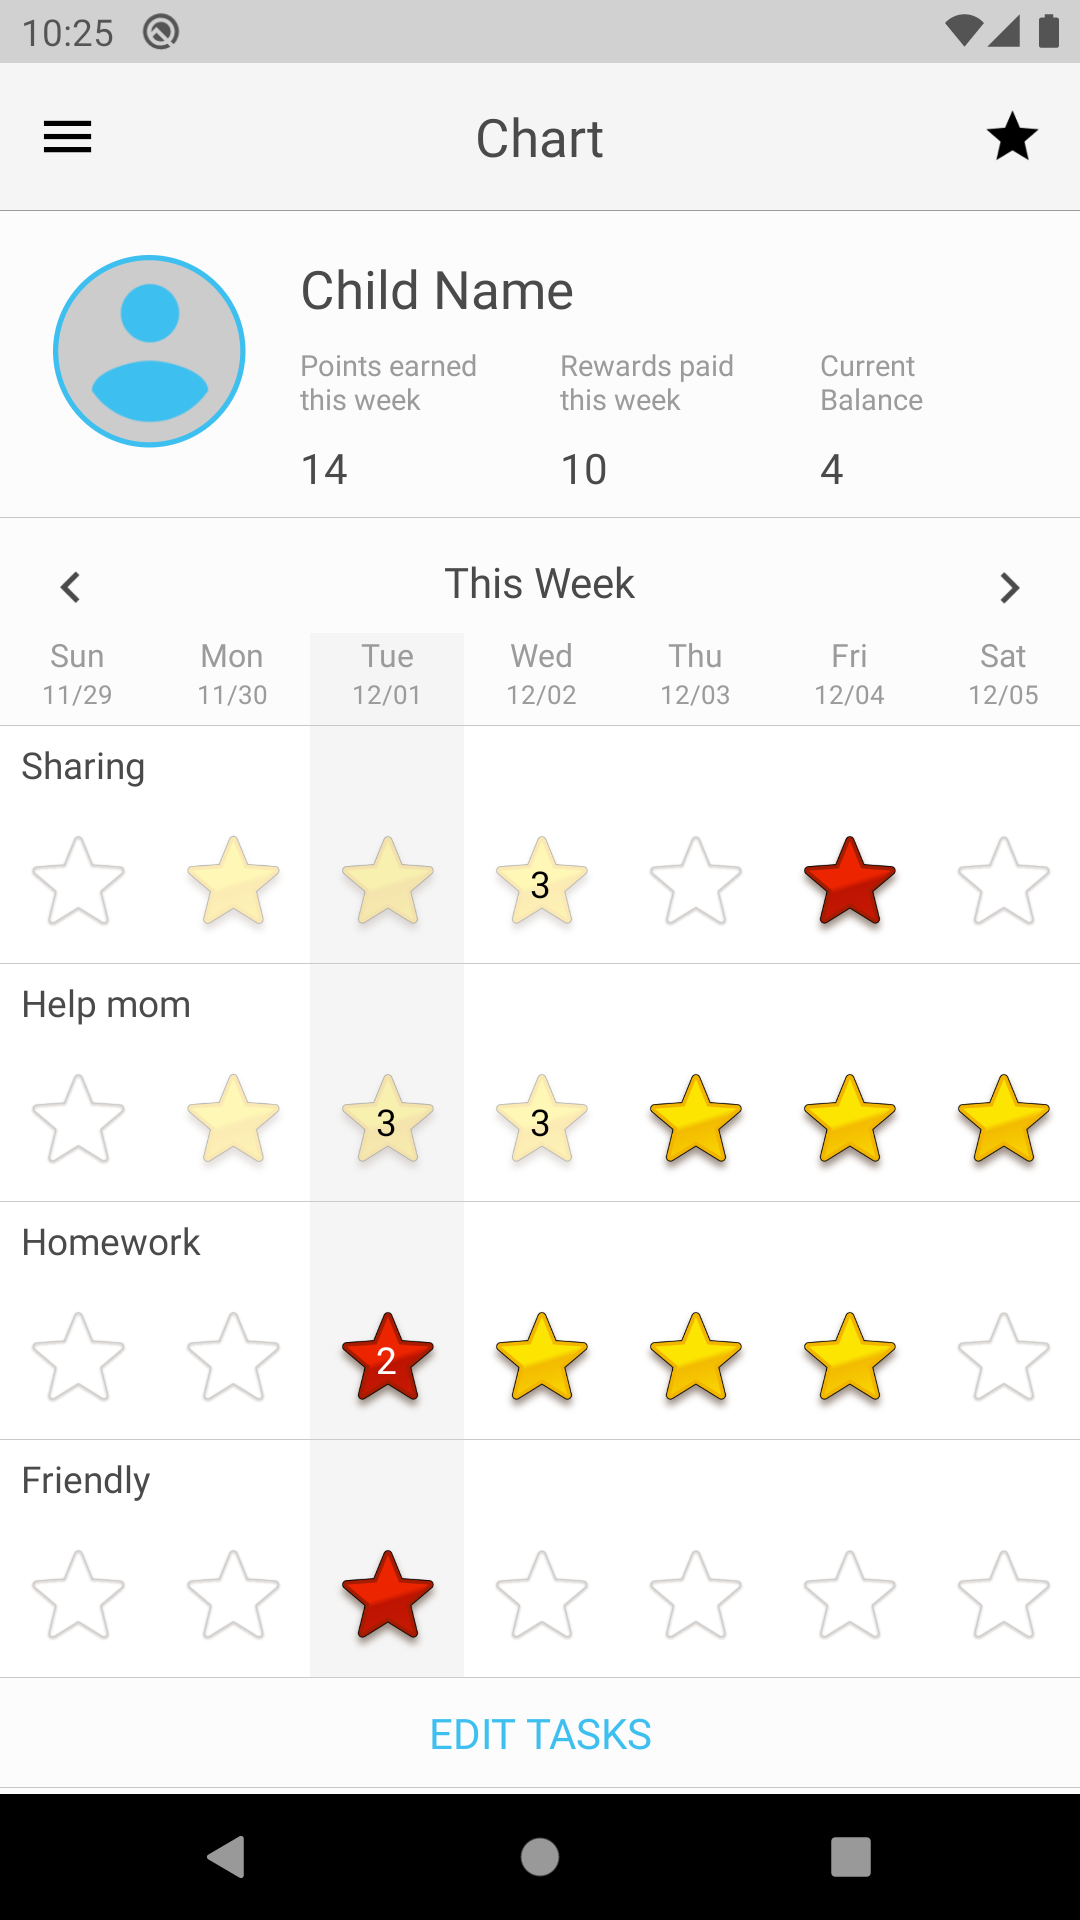
\includegraphics[width=.4\linewidth]{images/applications/iRewardChart/iRewardChart_1.png}} &
\subcaptionbox{Children list}{ 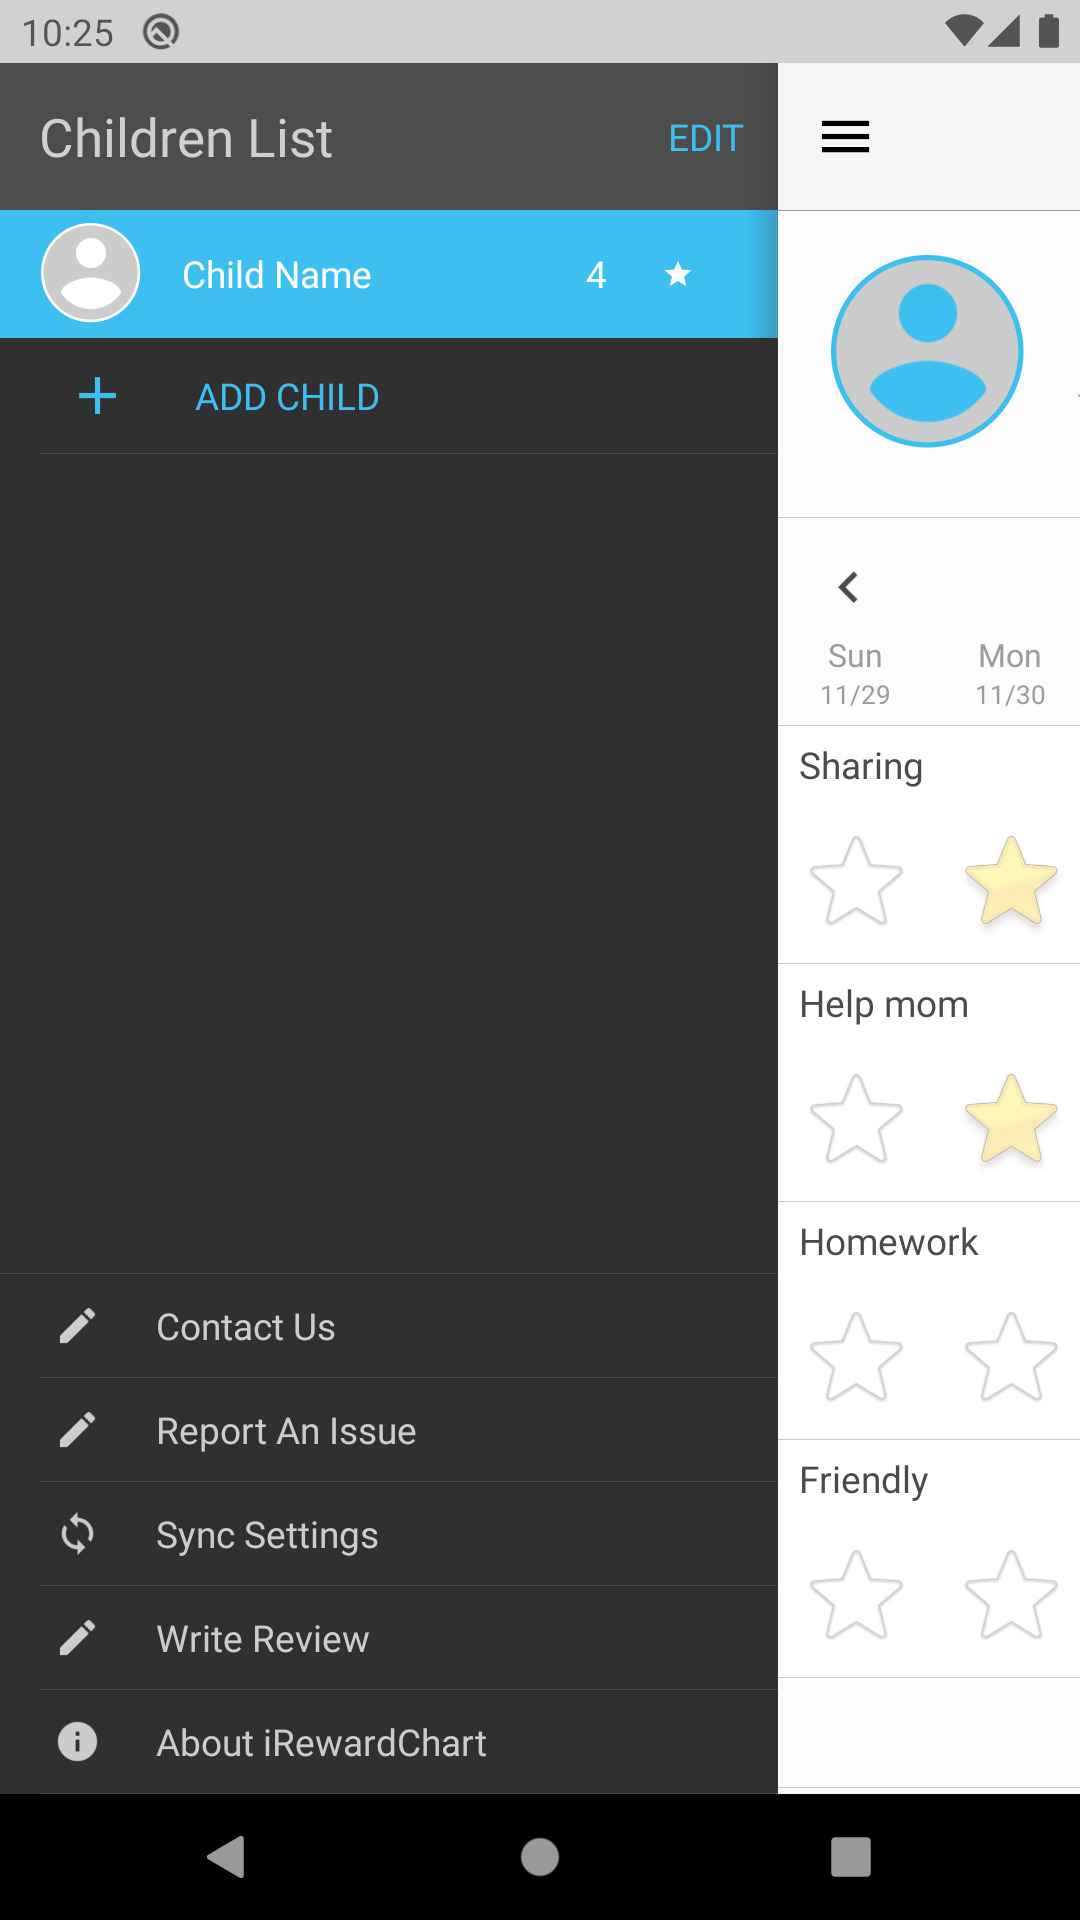
\includegraphics[width=.4\linewidth]{images/applications/iRewardChart/iRewardChart_2.png}} \\\\
\subcaptionbox{Tasks list}{ 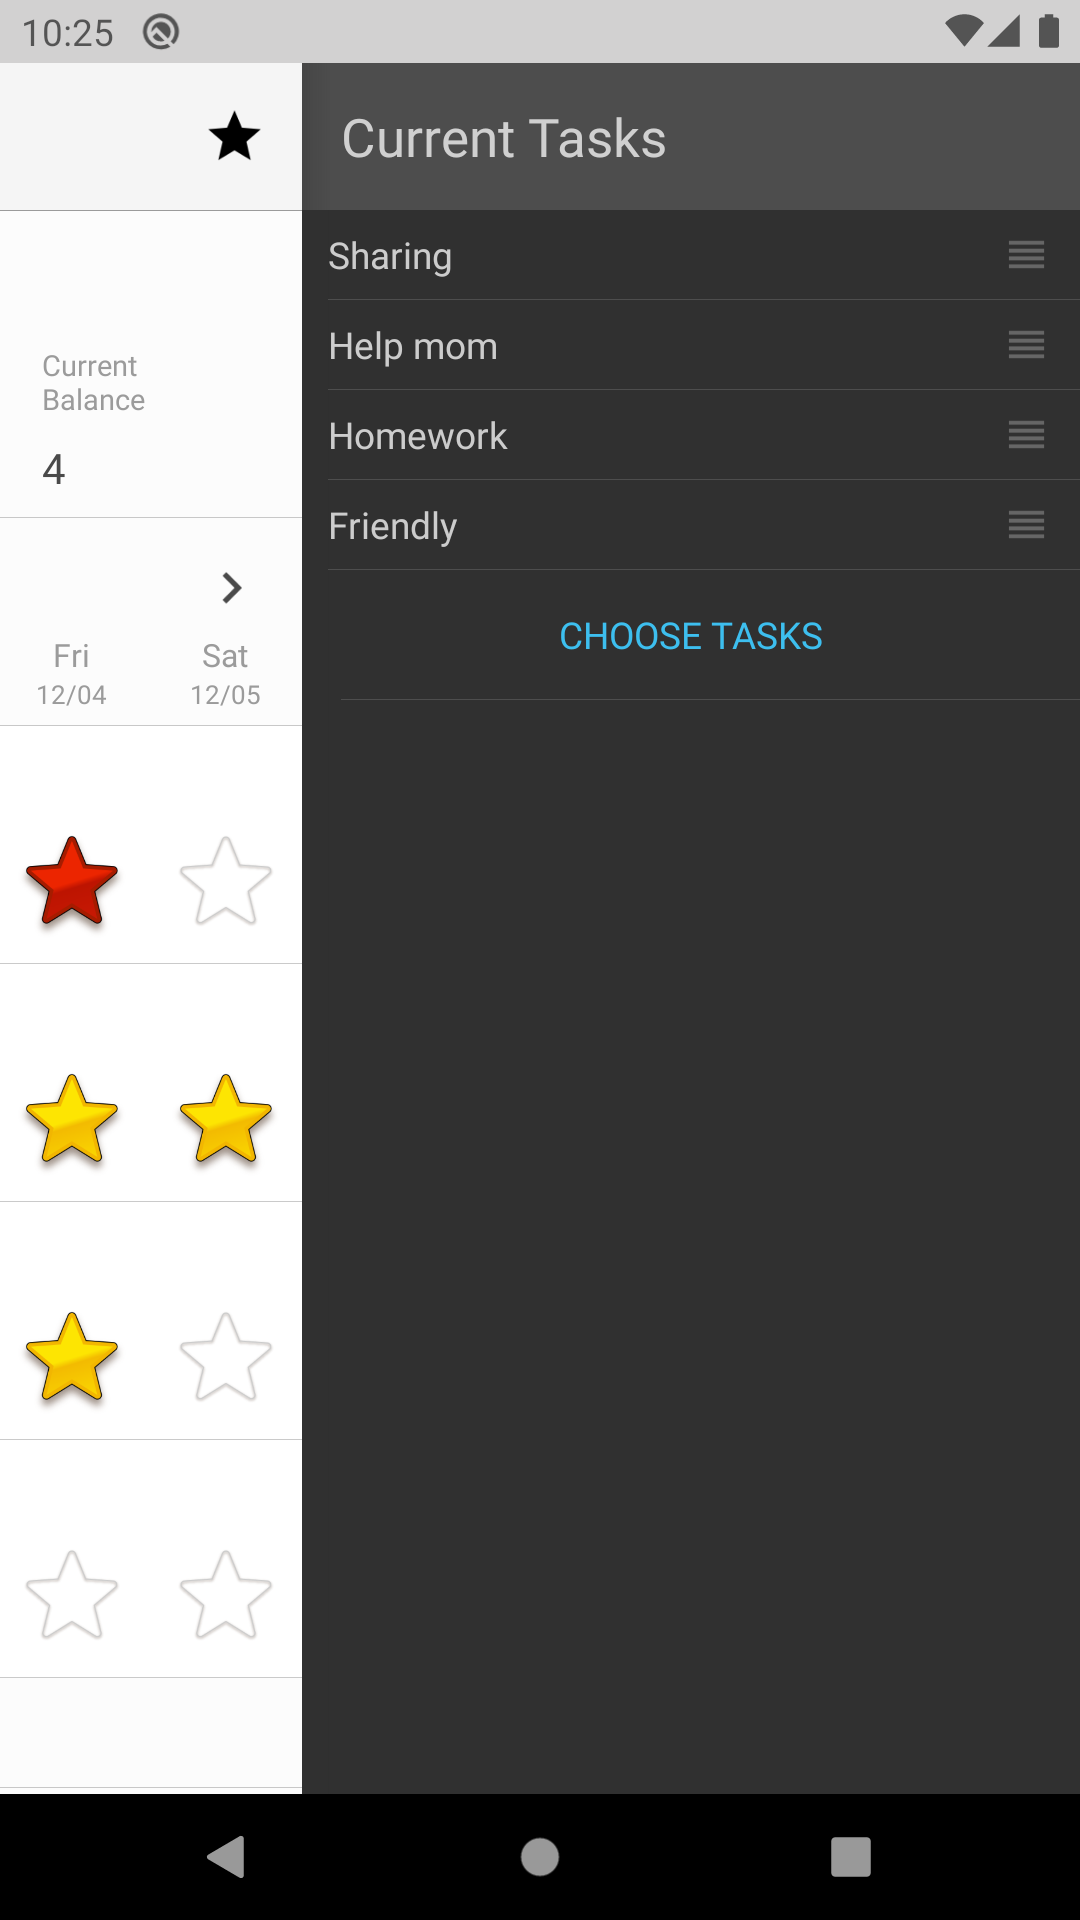
\includegraphics[width=.4\linewidth]{images/applications/iRewardChart/iRewardChart_3.png}} &
\subcaptionbox{Rewards list}{ 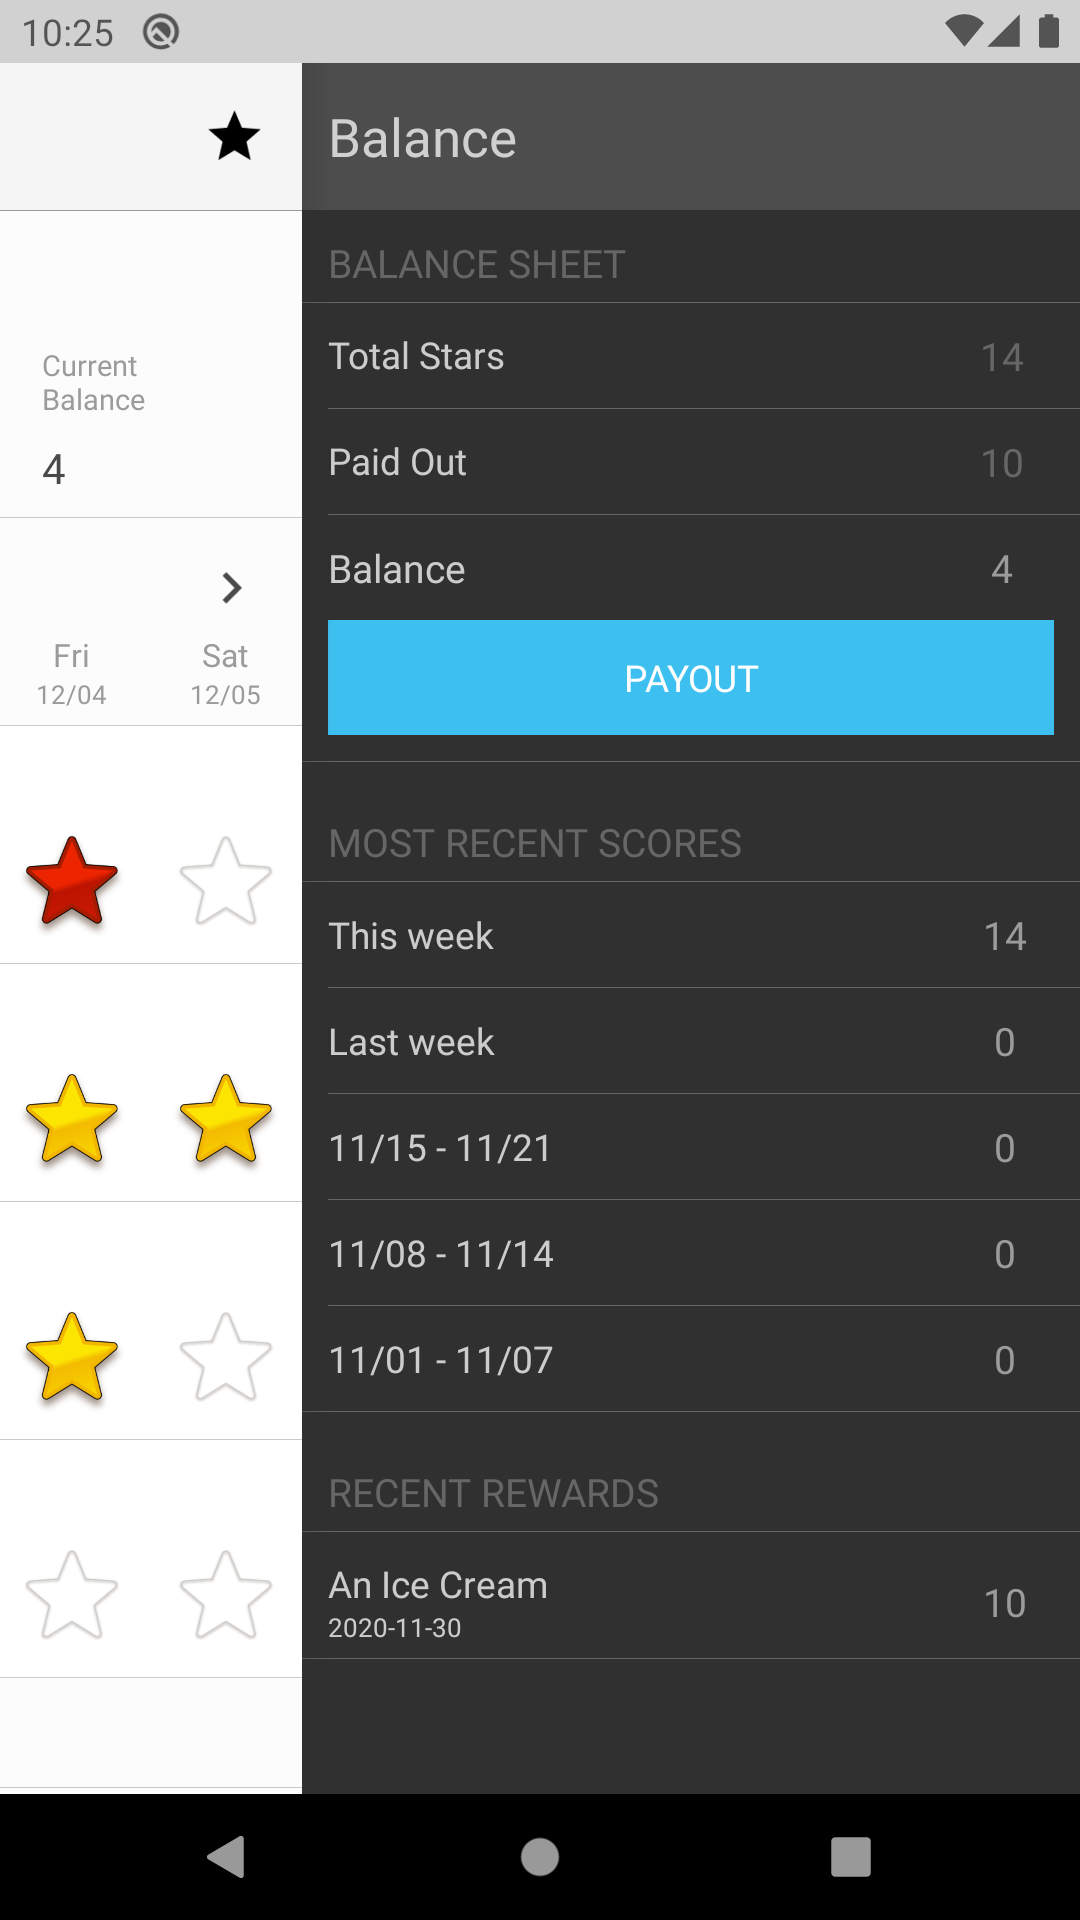
\includegraphics[width=.4\linewidth]{images/applications/iRewardChart/iRewardChart_4.png}}
\end{tabular}
\caption{\textit{iRewardChart} application screenshots}
\label{fig:applications:irewardchart}
\end{figure}

\begin{table}[htb]
\begin{tabularx}{\linewidth}{>{\parskip1ex}X@{\kern4\tabcolsep}>{\parskip1ex}X}
\toprule
\hfil\bfseries Advantages
&
\hfil\bfseries Disadvantages
\\
\cmidrule(r{3\tabcolsep}){1-1}\cmidrule(l{-\tabcolsep}){2-2}

Available on both platforms\par
Small application size\par
Older Android versions support

&

Low Google Play rating\par
Not updated for a long time\par
Cumbersome design\par
Poor user experience\par
Not many options in the free version\par
No child's perspective

\\
\bottomrule
\end{tabularx}
\caption{\textit{iRewardChart} application advantages and disadvantages}
\label{tab:applications:irewardchart}
\end{table}


\subsection{ChorePad}\label{subsec:market:solutions:chorepad}
\textit{ChorePad} \cite{ChorePadLite,ChorePadChores} has two different versions, paid and free, distributed as separate applications. It targets children aged four and older. The application supports only Apple devices with iOS version 9.0 or later. Apple App Store does not share the downloads number or the last update date, therefore, it is difficult to estimate it. The free version has a rating of 2.9 and the paid one - 4.4. Both versions have a size in range 60-70MB.
\\\\
The application has a child-friendly, though occasionally confusing design. It also allows for Despite provided onboarding mechanisms, it is not always straightforward to use. Its main screen represents a board with children profiles, with only one available in the free version. \textit{Chores}, because this is the name of tasks, are the main focal point in the application (however, only four are available in the free version). Rewards functionality, even if available, is marginal. Application has a child's perspective; however, it does not change elements visibility, but only editing functionality.
\\\\
Example screenshots of the \textit{ChorePad} application were presented in Figure~\ref{fig:applications:chorepad}. A summary of its strengths and weaknesses was presented in Table~\ref{tab:applications:chorepad}.
\\
\begin{figure}
\centering
\begin{tabular}{cc}
\subcaptionbox{Children list (main screen)}{ 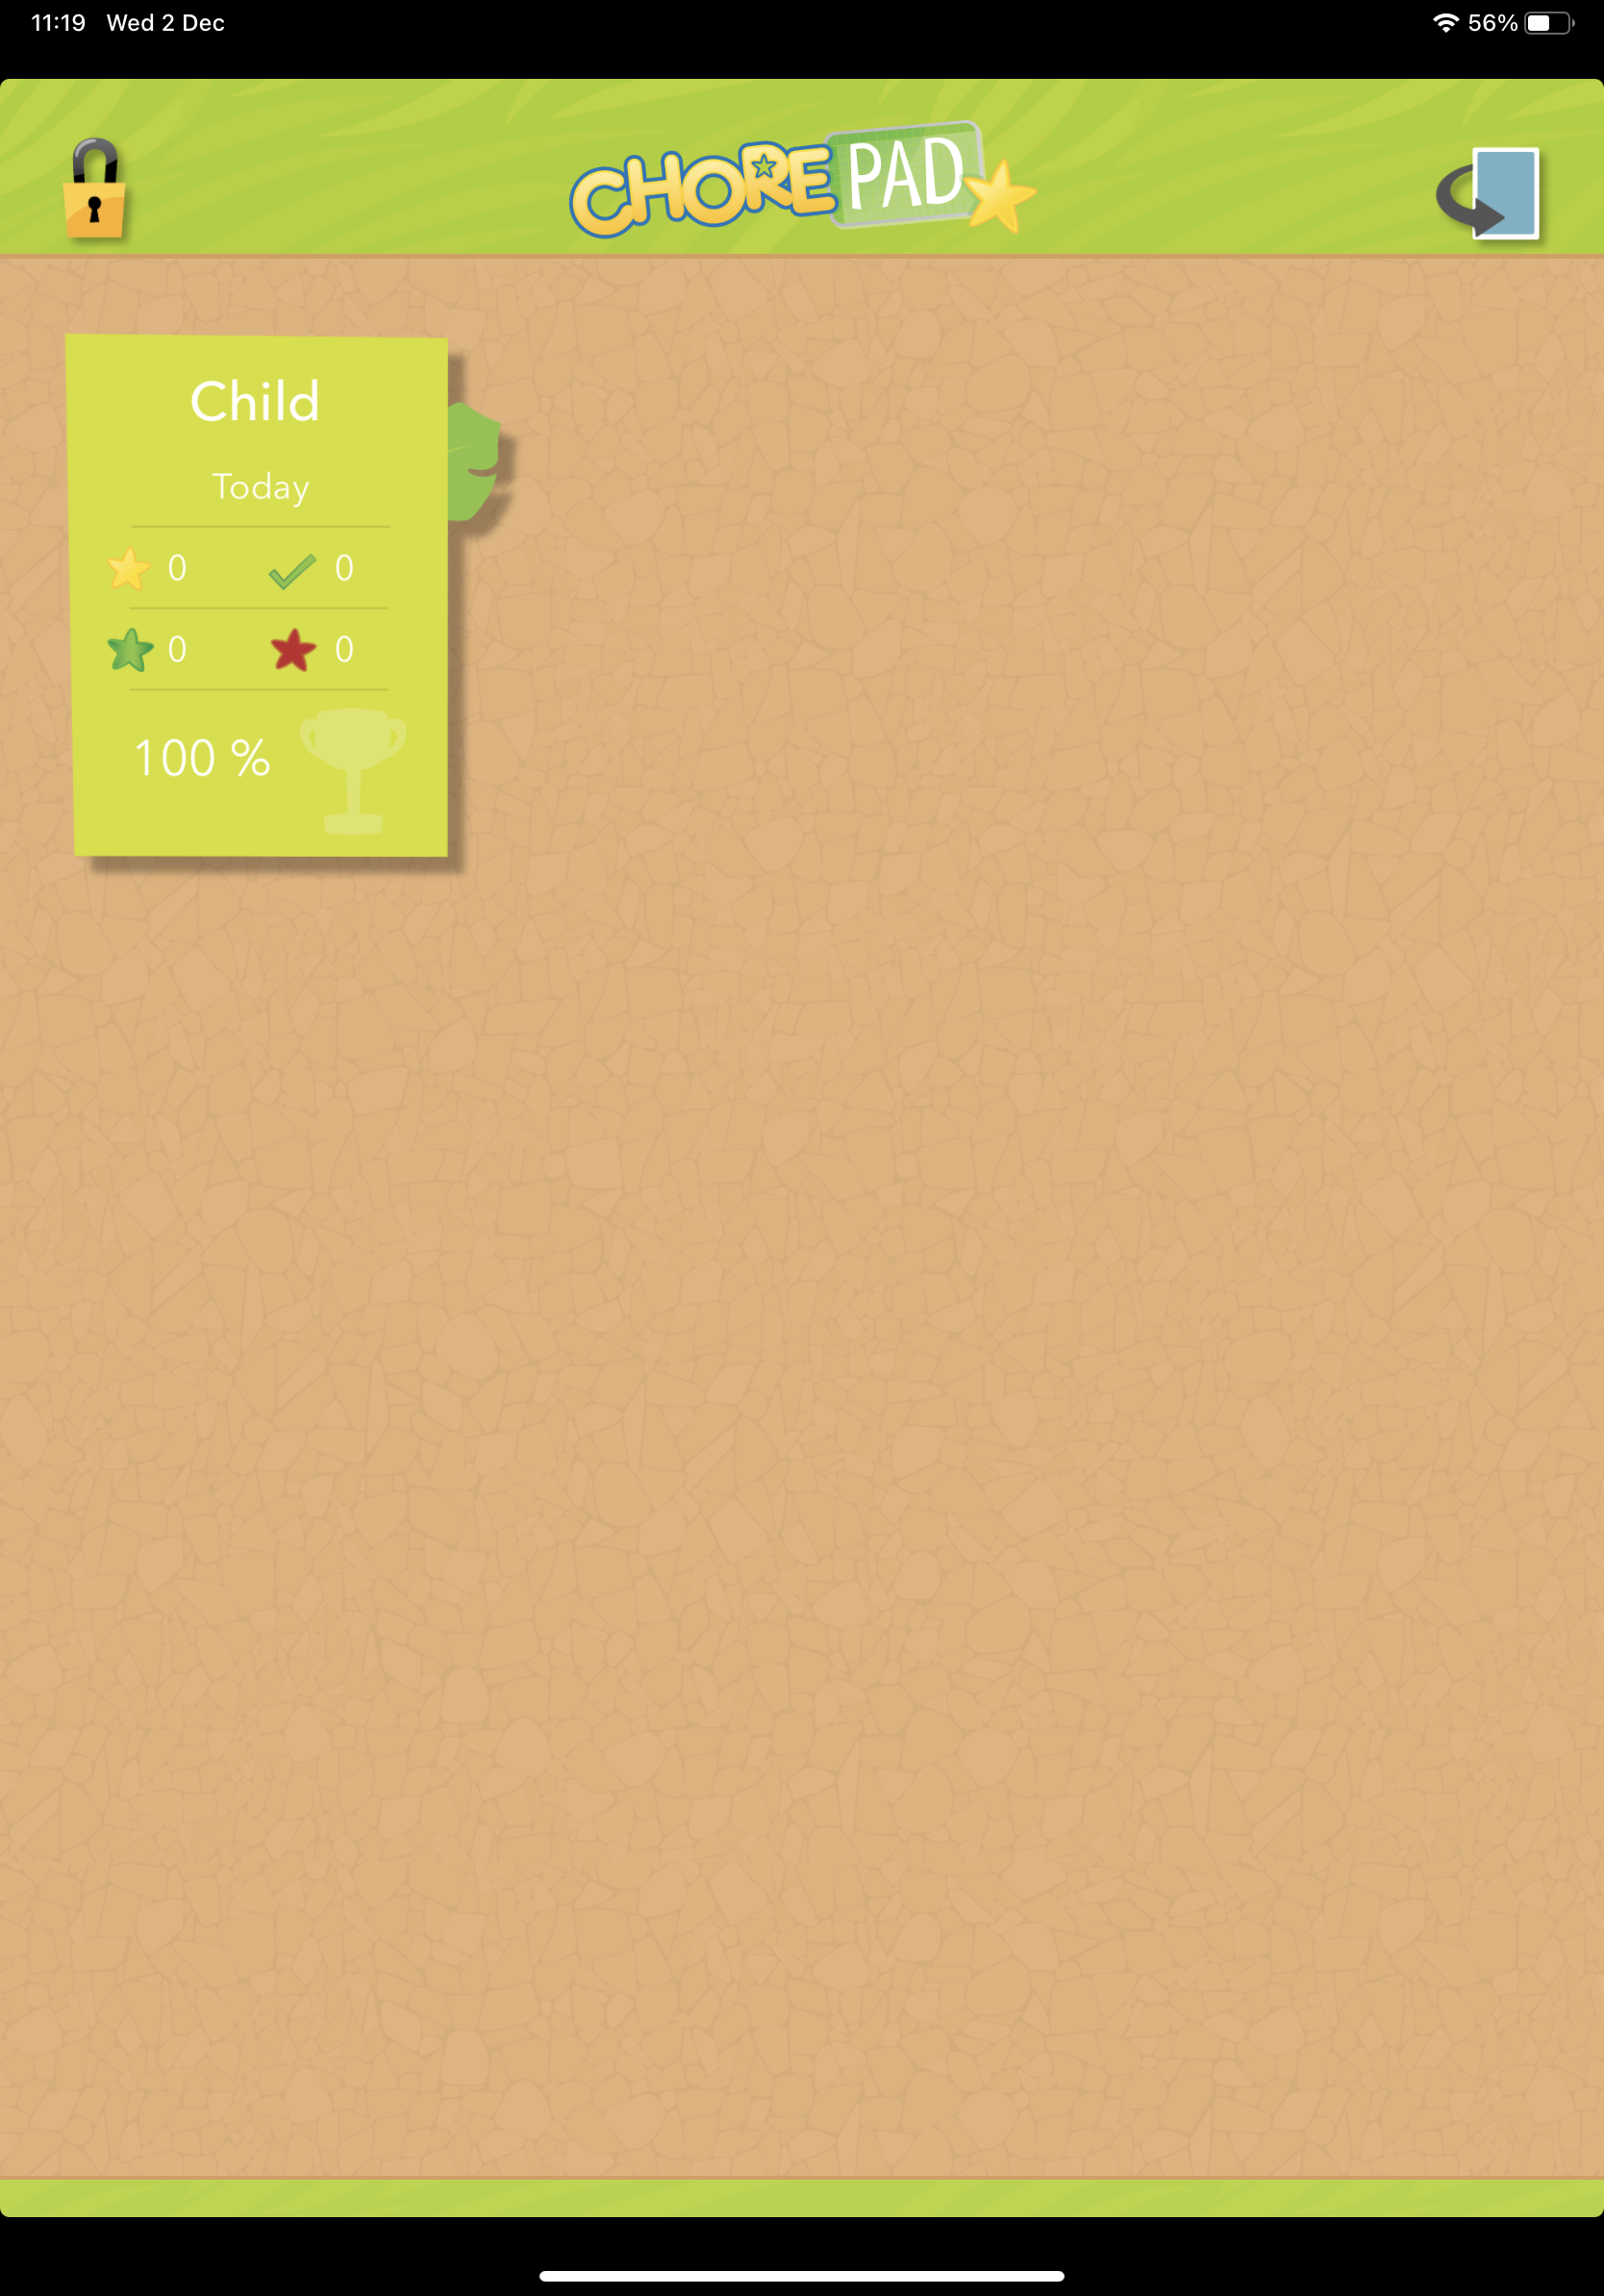
\includegraphics[width=.45\linewidth]{images/applications/ChorePad/ChorePad_1.png}} &
\subcaptionbox{Chores list}{ 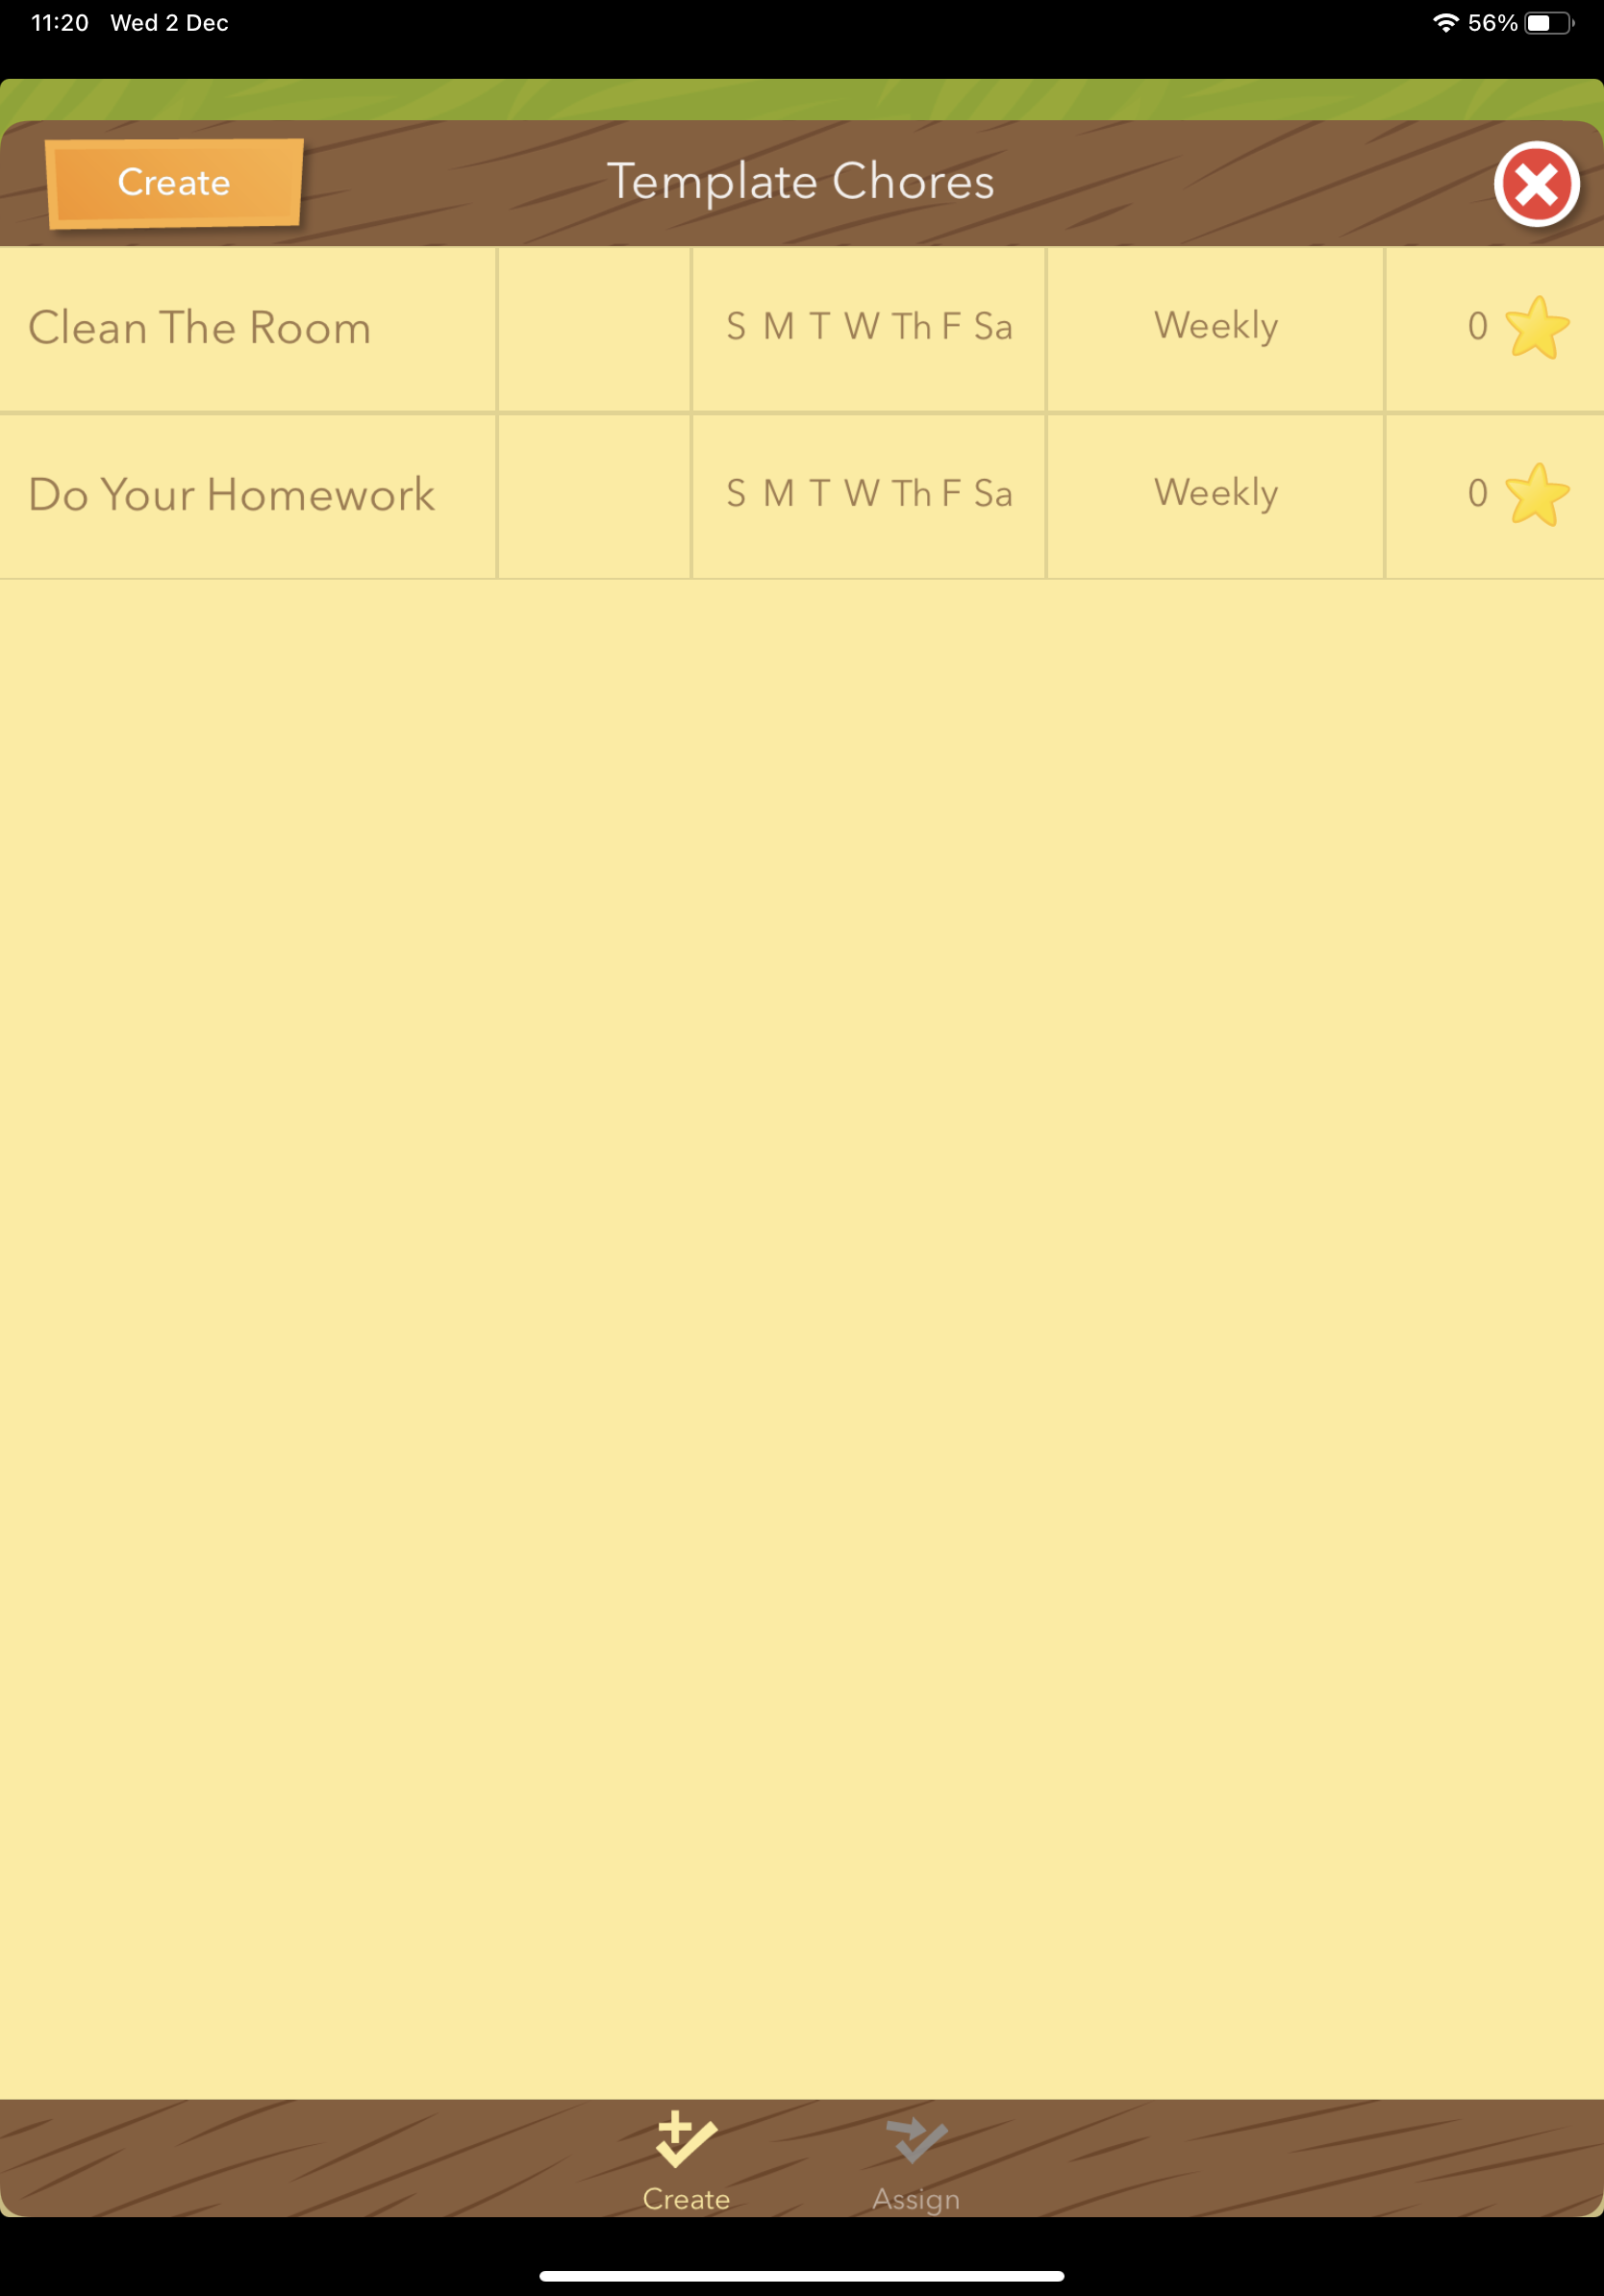
\includegraphics[width=.45\linewidth]{images/applications/ChorePad/ChorePad_2.png}} \\\\\\\\
\subcaptionbox{Child view}{ 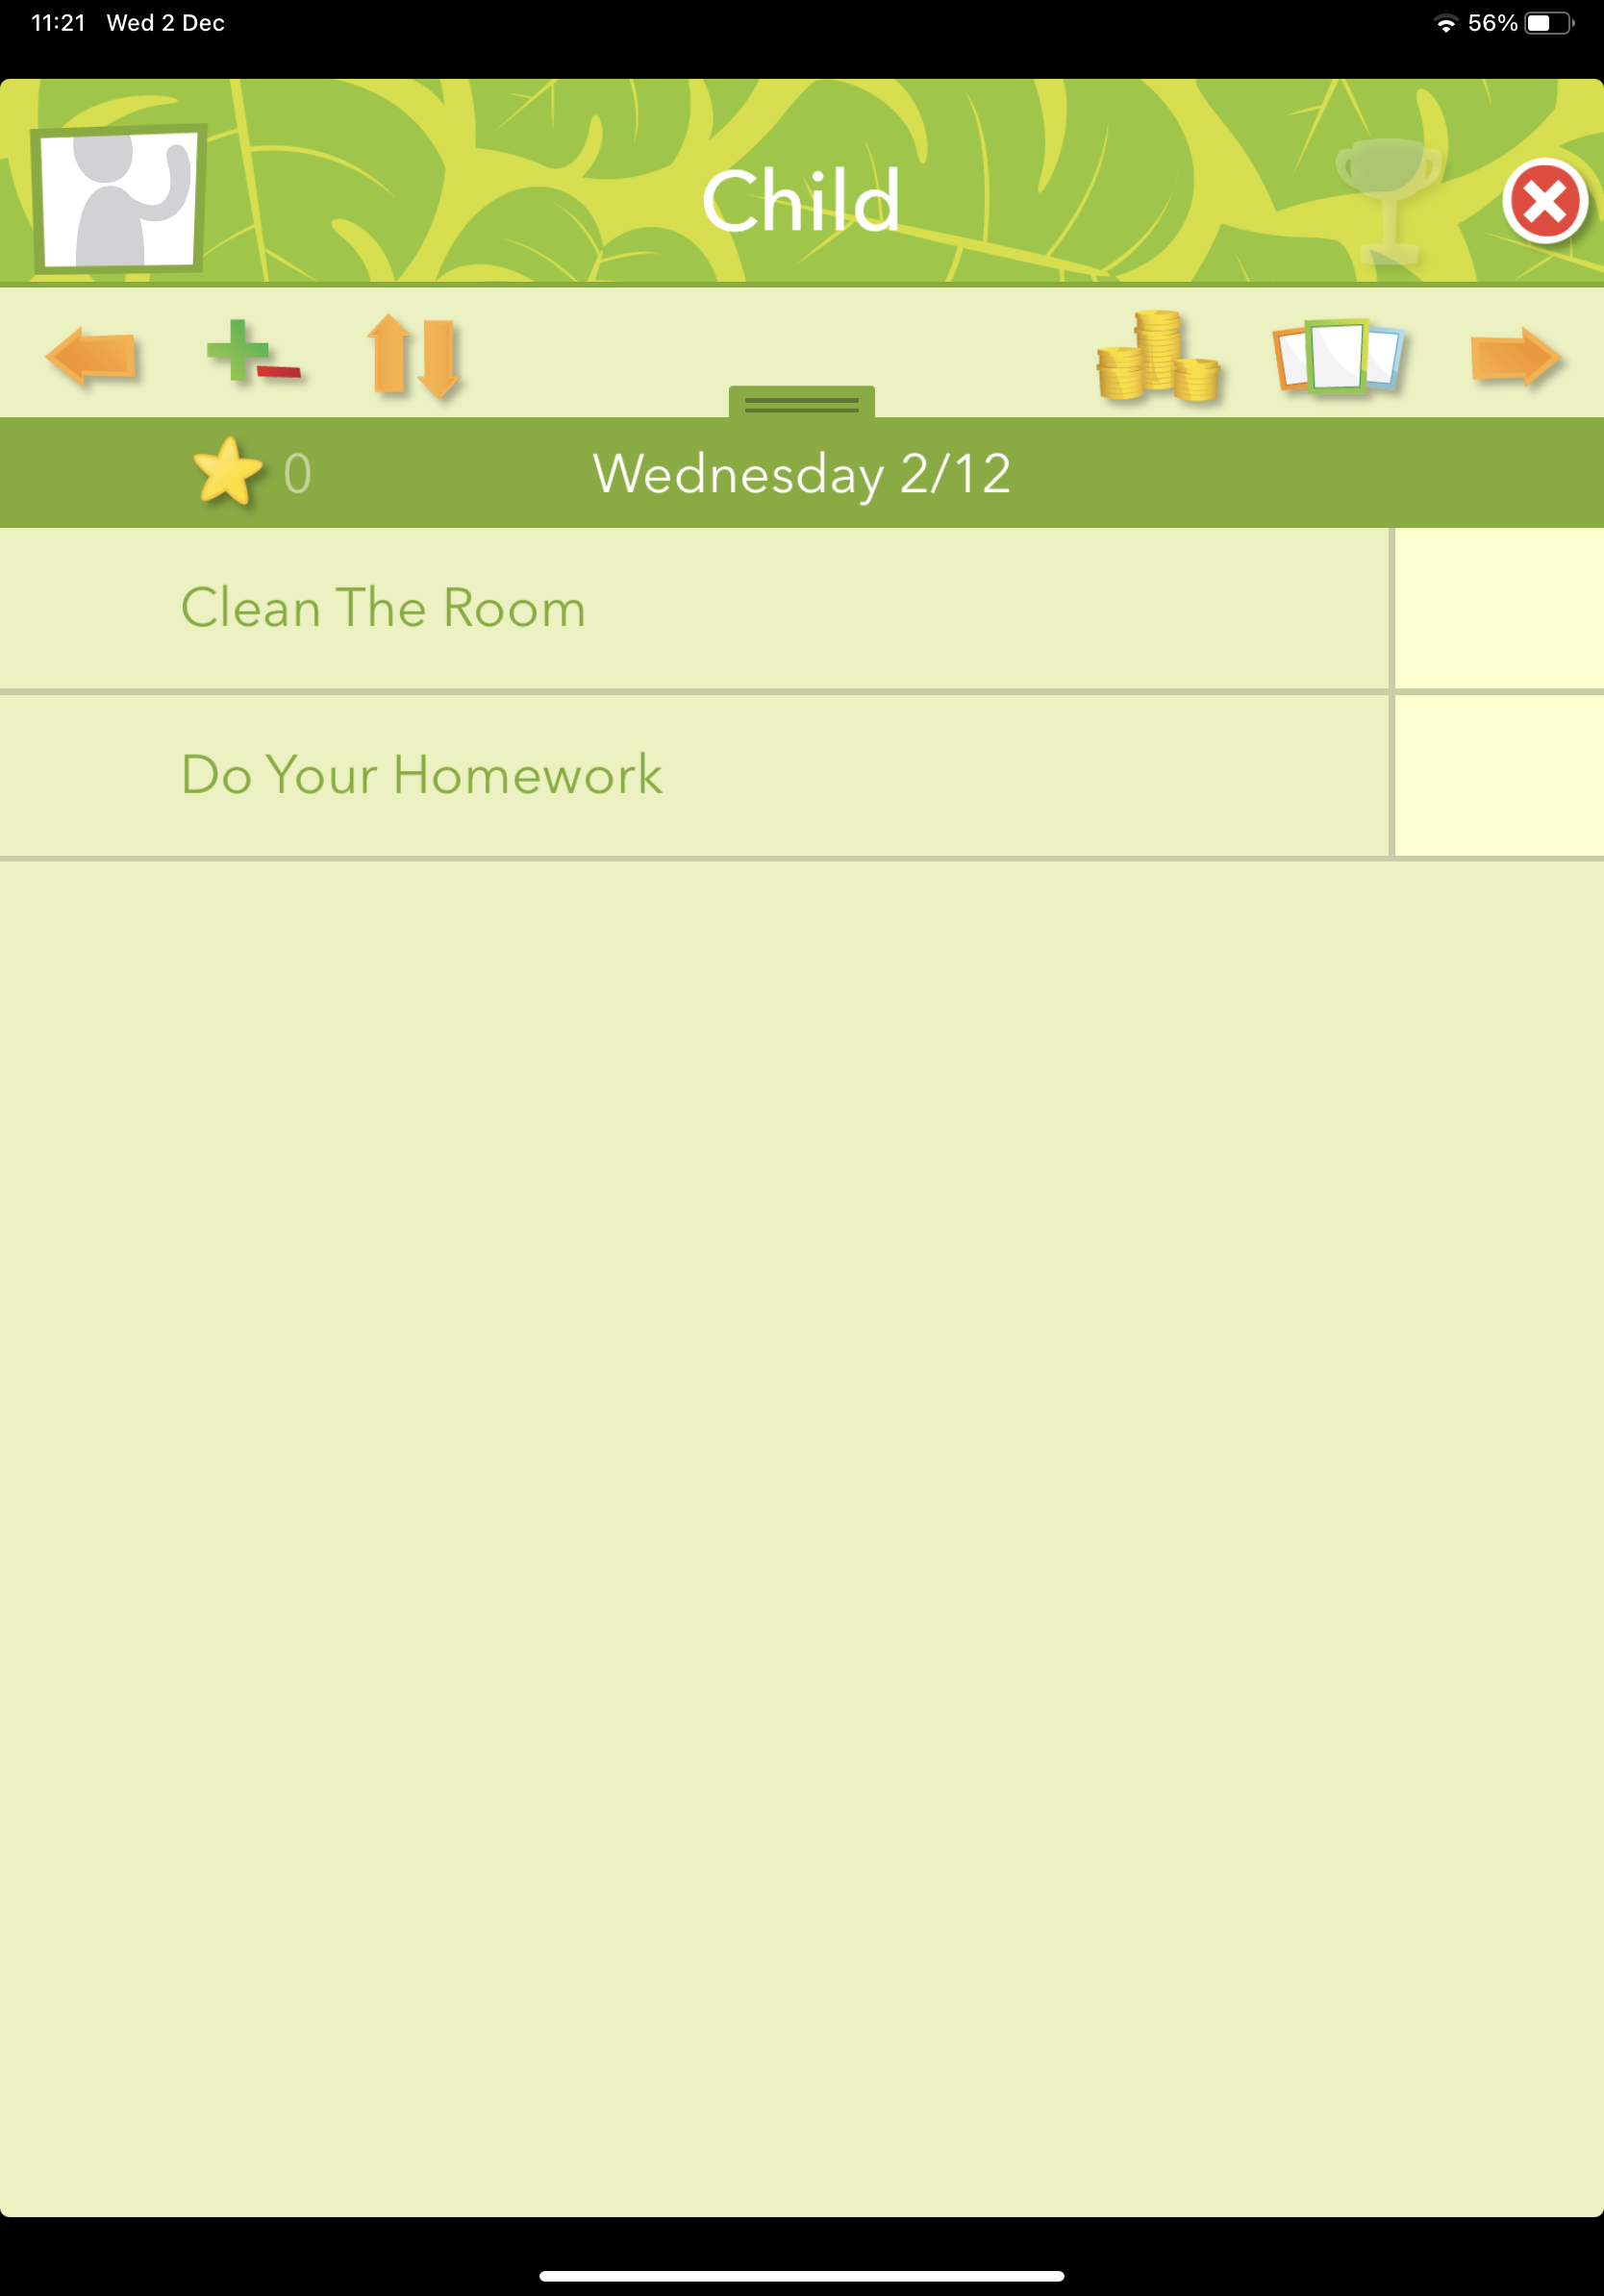
\includegraphics[width=.45\linewidth]{images/applications/ChorePad/ChorePad_3.png}} &
\subcaptionbox{Theme customization}{ 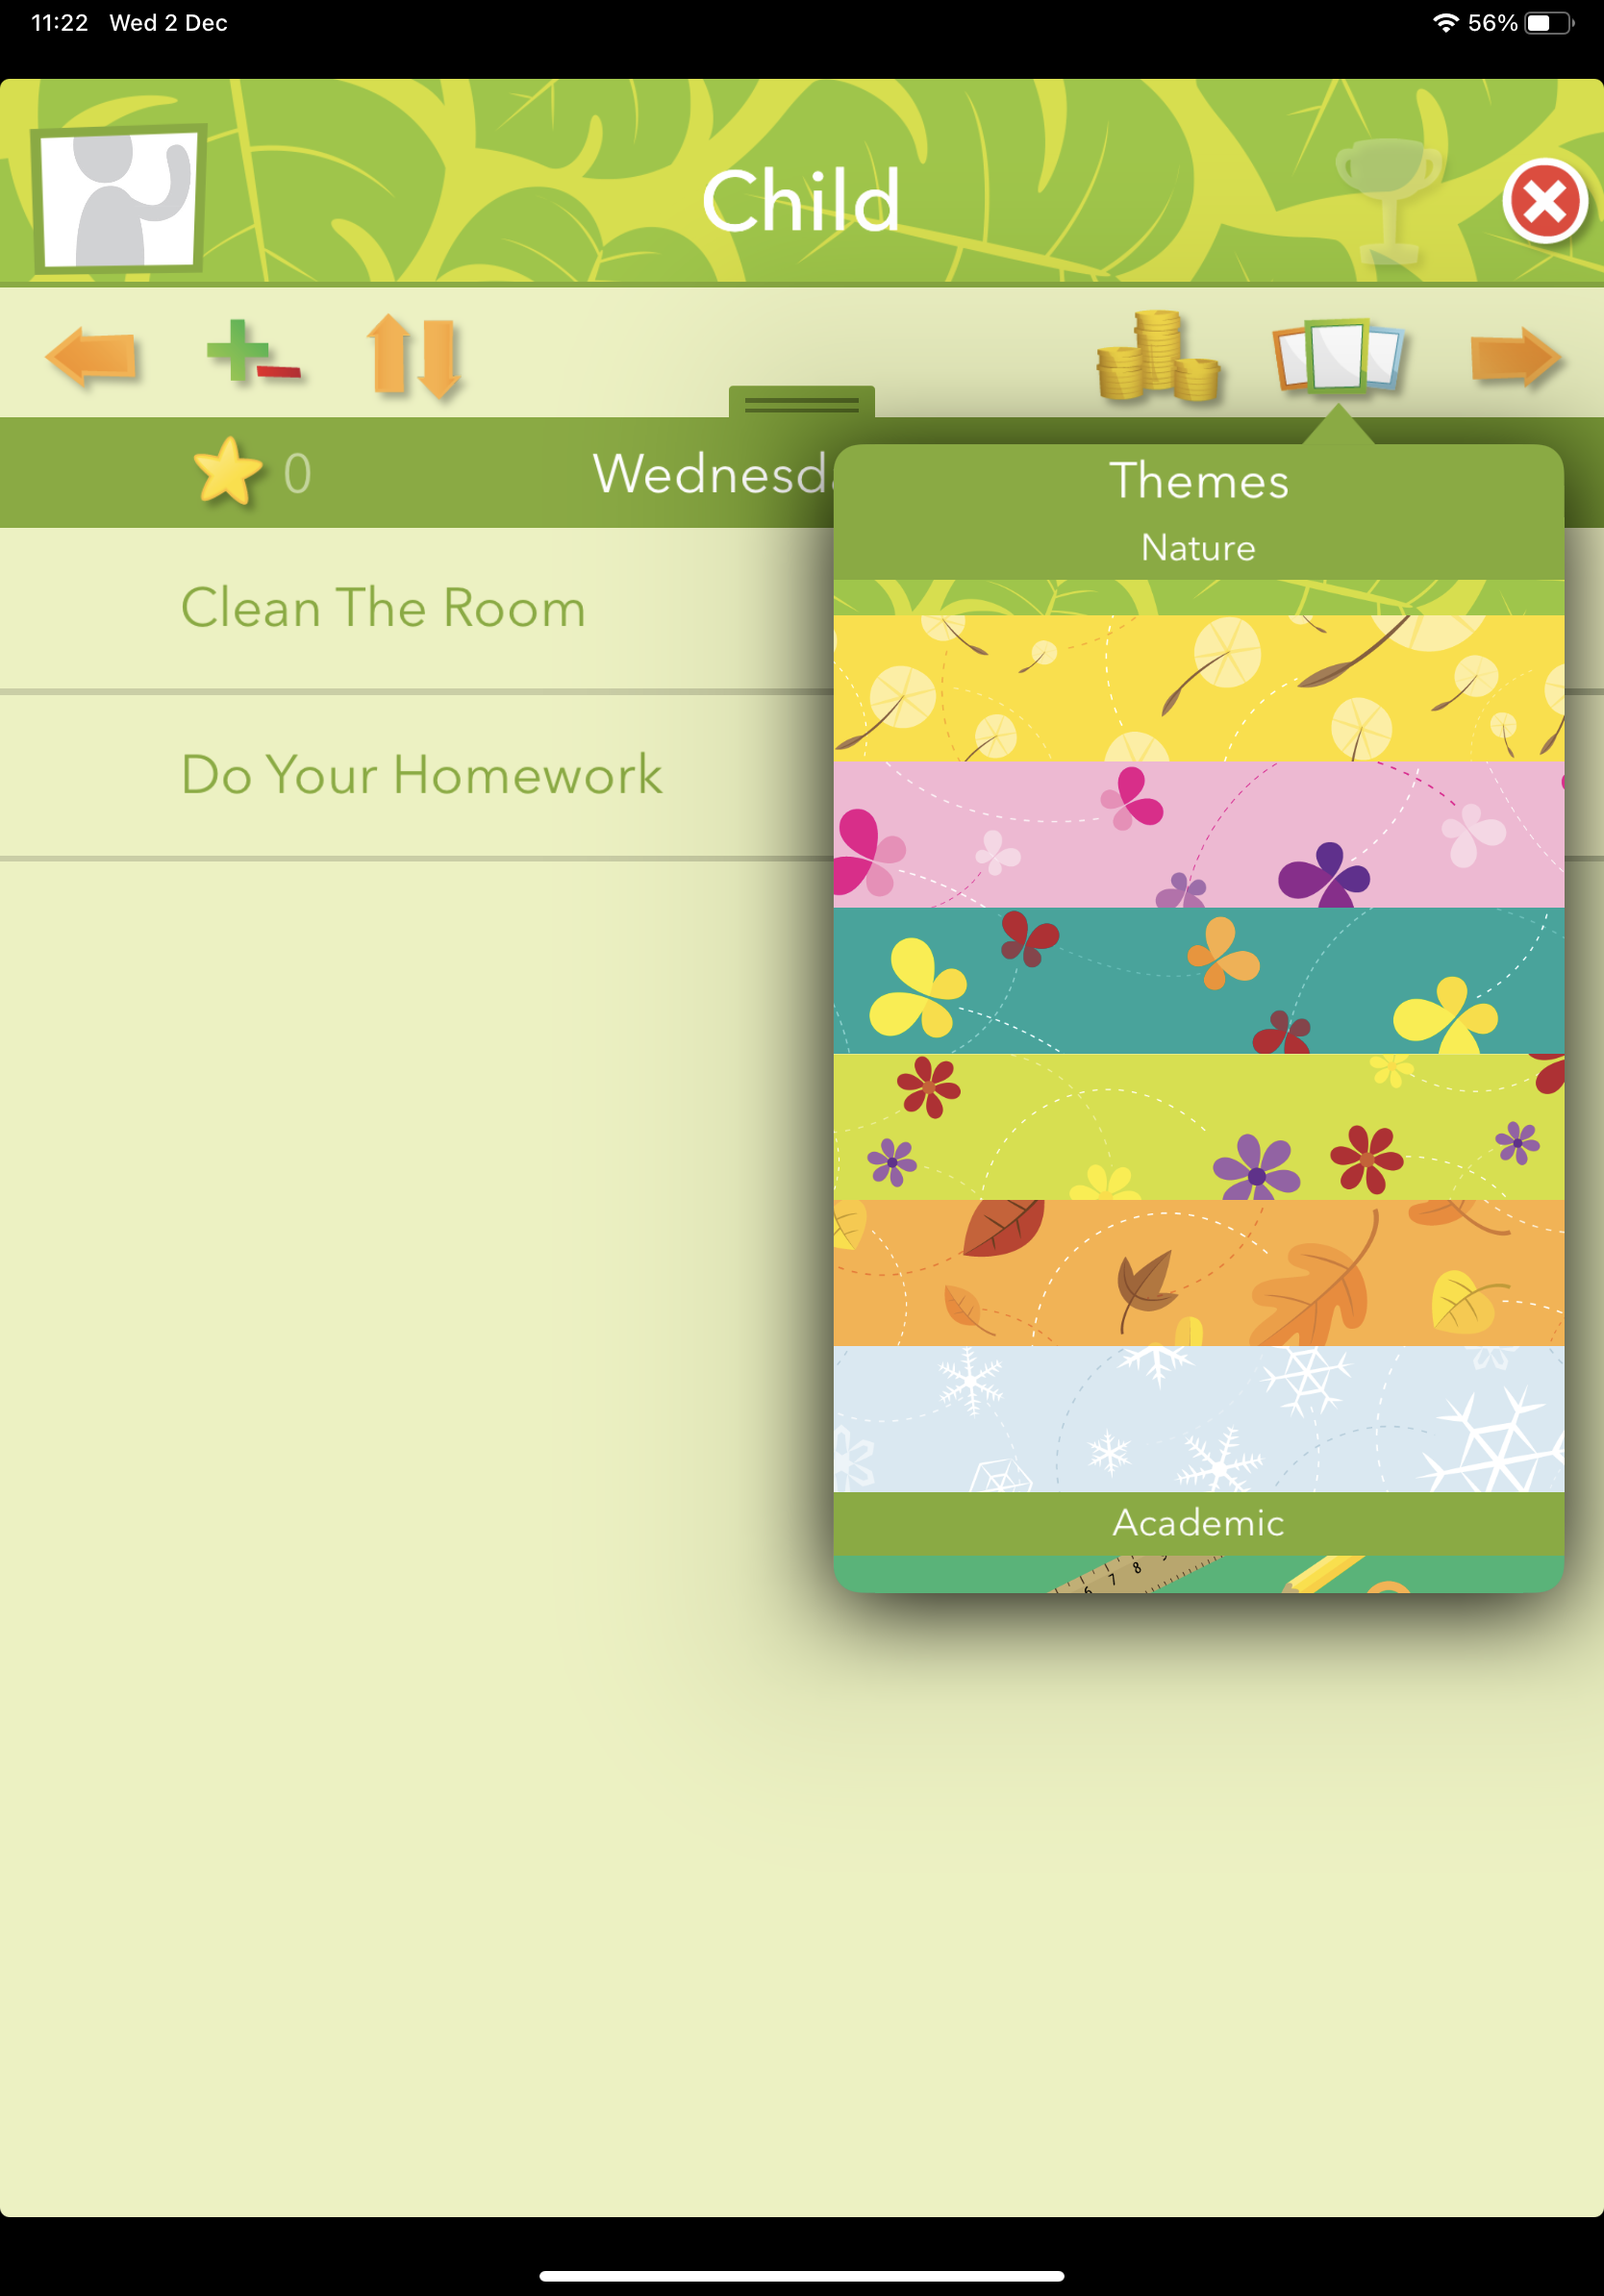
\includegraphics[width=.45\linewidth]{images/applications/ChorePad/ChorePad_4.png}}
\end{tabular}
\caption{\textit{ChorePad} application screenshots}
\label{fig:applications:chorepad}
\end{figure}

\begin{table}[htb]
\begin{tabularx}{\linewidth}{>{\parskip1ex}X@{\kern4\tabcolsep}>{\parskip1ex}X}
\toprule
\hfil\bfseries Advantages
&
\hfil\bfseries Disadvantages
\\
\cmidrule(r{3\tabcolsep}){1-1}\cmidrule(l{-\tabcolsep}){2-2}

Available on both platforms\par
Child-friendly, customizable design

&

Separate free and paid versions\par
Low Apple App store rating\par
Available just on iOS platform\par
Quite big application size\par
Occasionally confusing design\par
Not many options in the free version

\\
\bottomrule
\end{tabularx}
\caption{\textit{ChorePad} application advantages and disadvantages}
\label{tab:applications:chorepad}
\end{table}


\subsection{Homey - Chores and Allowance}\label{subsec:market:solutions:homey}
\textit{Homey - Chores and Allowance} \cite{HomeyChoresAllowance,HomeyChoresAllowancea} (later referred to as \textit{Homey}) is an application available on both Android and iOS operating systems. The application does not have an age limit and is targeted to everyone. It rates 2.8 on Google Play, has more than 50000 downloads, and its size is 27MB. It needs Android version 4.1 or higher to run correctly. The last update was released in February 2020.
\\\\
Application is much more complex than the previous two. It has many options, including two different types of tasks (\textit{jobs} and \textit{responsibilities}), pre-defined lists of tasks, in-family chat or even custom reports. Instead of rewards, one can set a weekly allowance that is paid to children once they meet their goals. It also supports switching between parent's and child's perspective. The design is tidy but tends to be over-engineered. \textit{Homey} crashes frequently, which is also pointed out by the community in the ratings.
\\\\
Example screenshots of the \textit{Homey} application were presented in Figure~\ref{fig:applications:homey}. A summary of its merits and demerits was presented in Table~\ref{tab:applications:homey}.
\\
\begin{figure}
\centering
\begin{tabular}{cc}
\subcaptionbox{Responsibilities list}{ 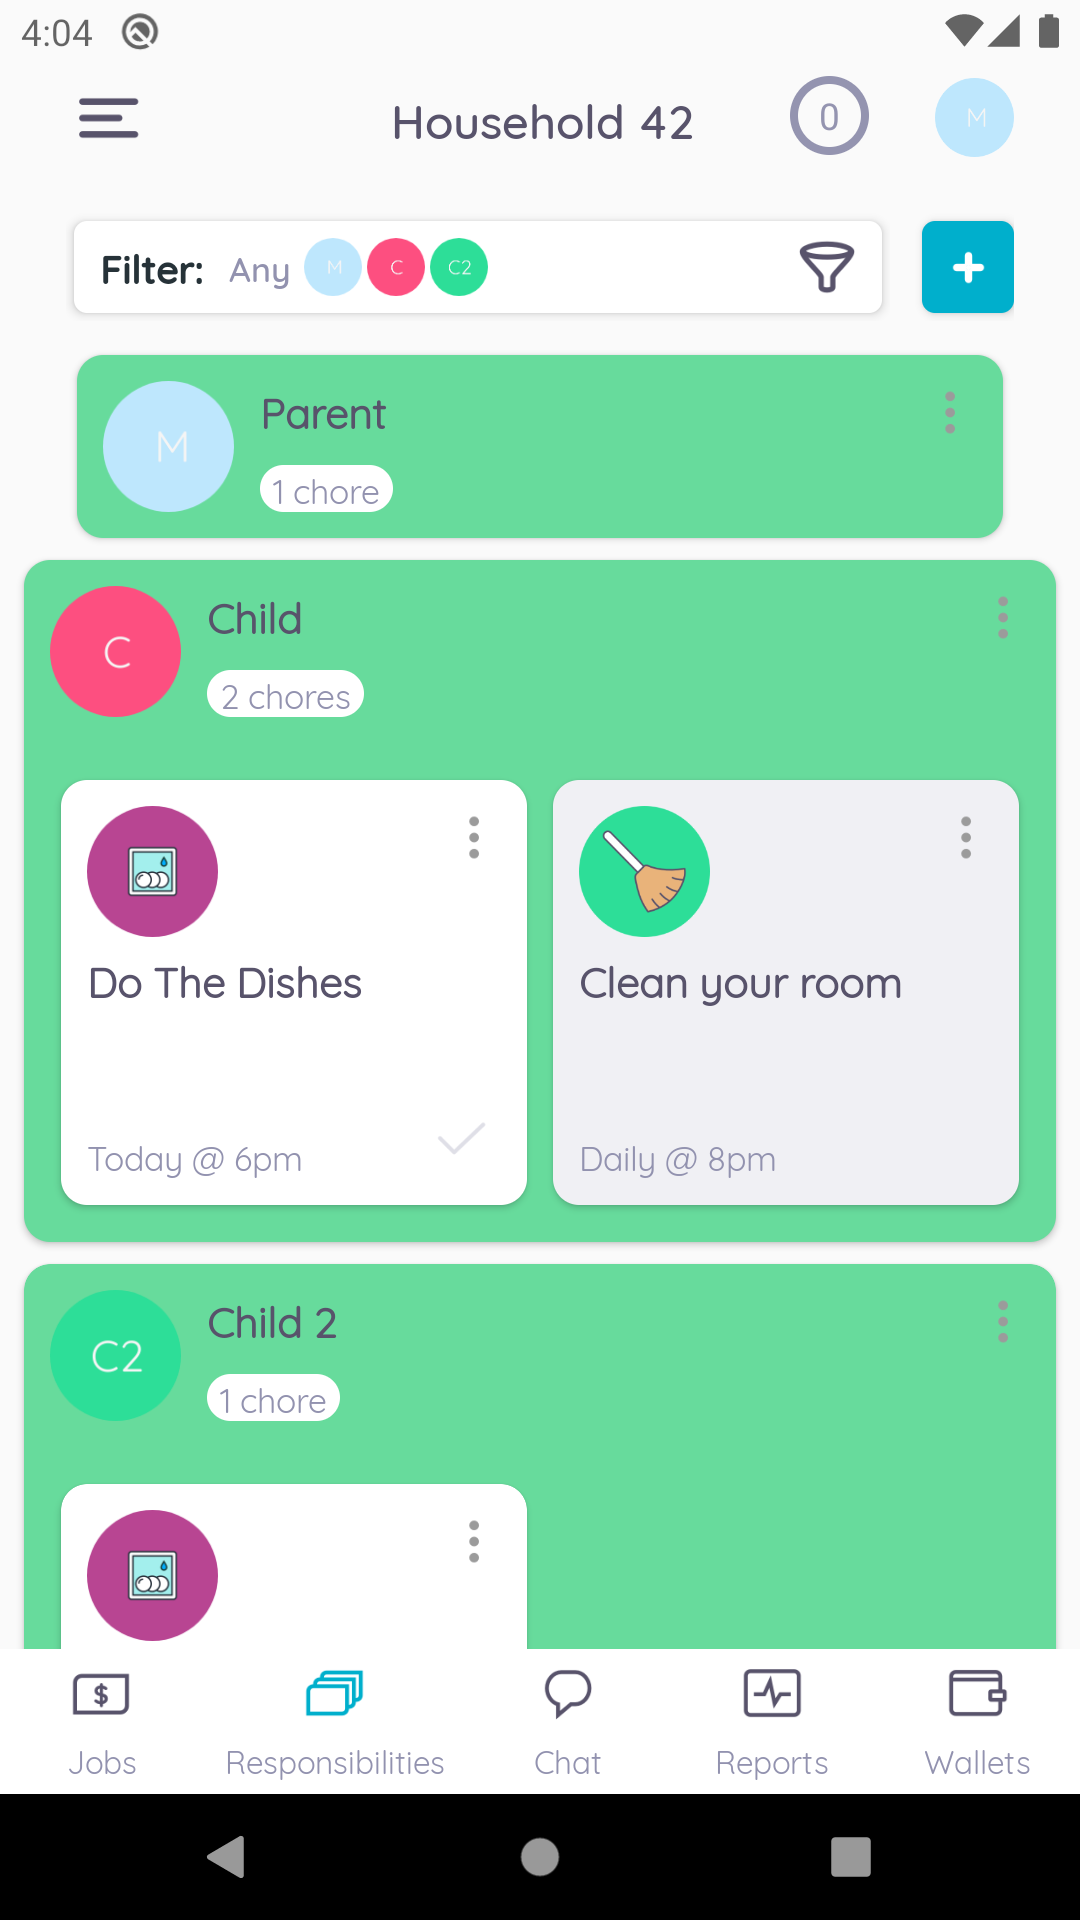
\includegraphics[width=.4\linewidth]{images/applications/Homey/Homey_1.png}} &
\subcaptionbox{In-family chat}{ 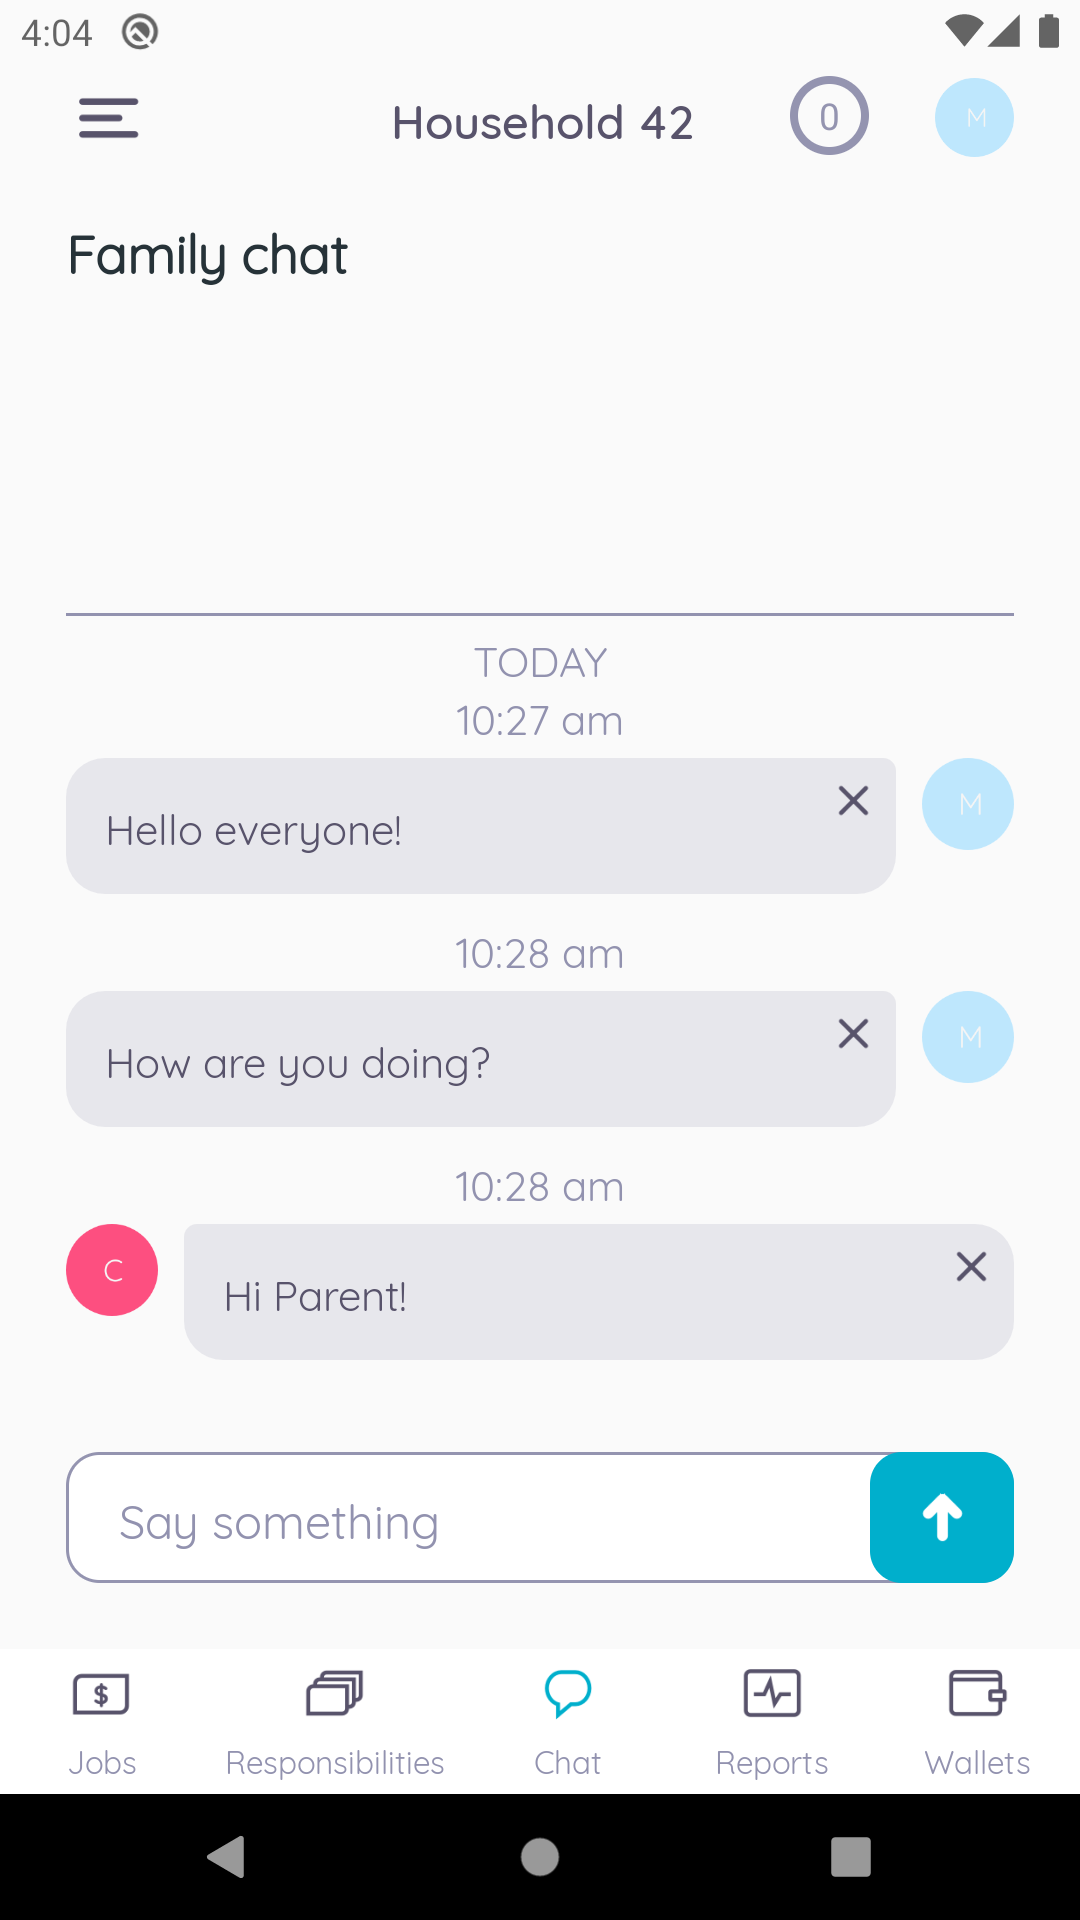
\includegraphics[width=.4\linewidth]{images/applications/Homey/Homey_2.png}} \\\\
\subcaptionbox{Allowance tracker}{ 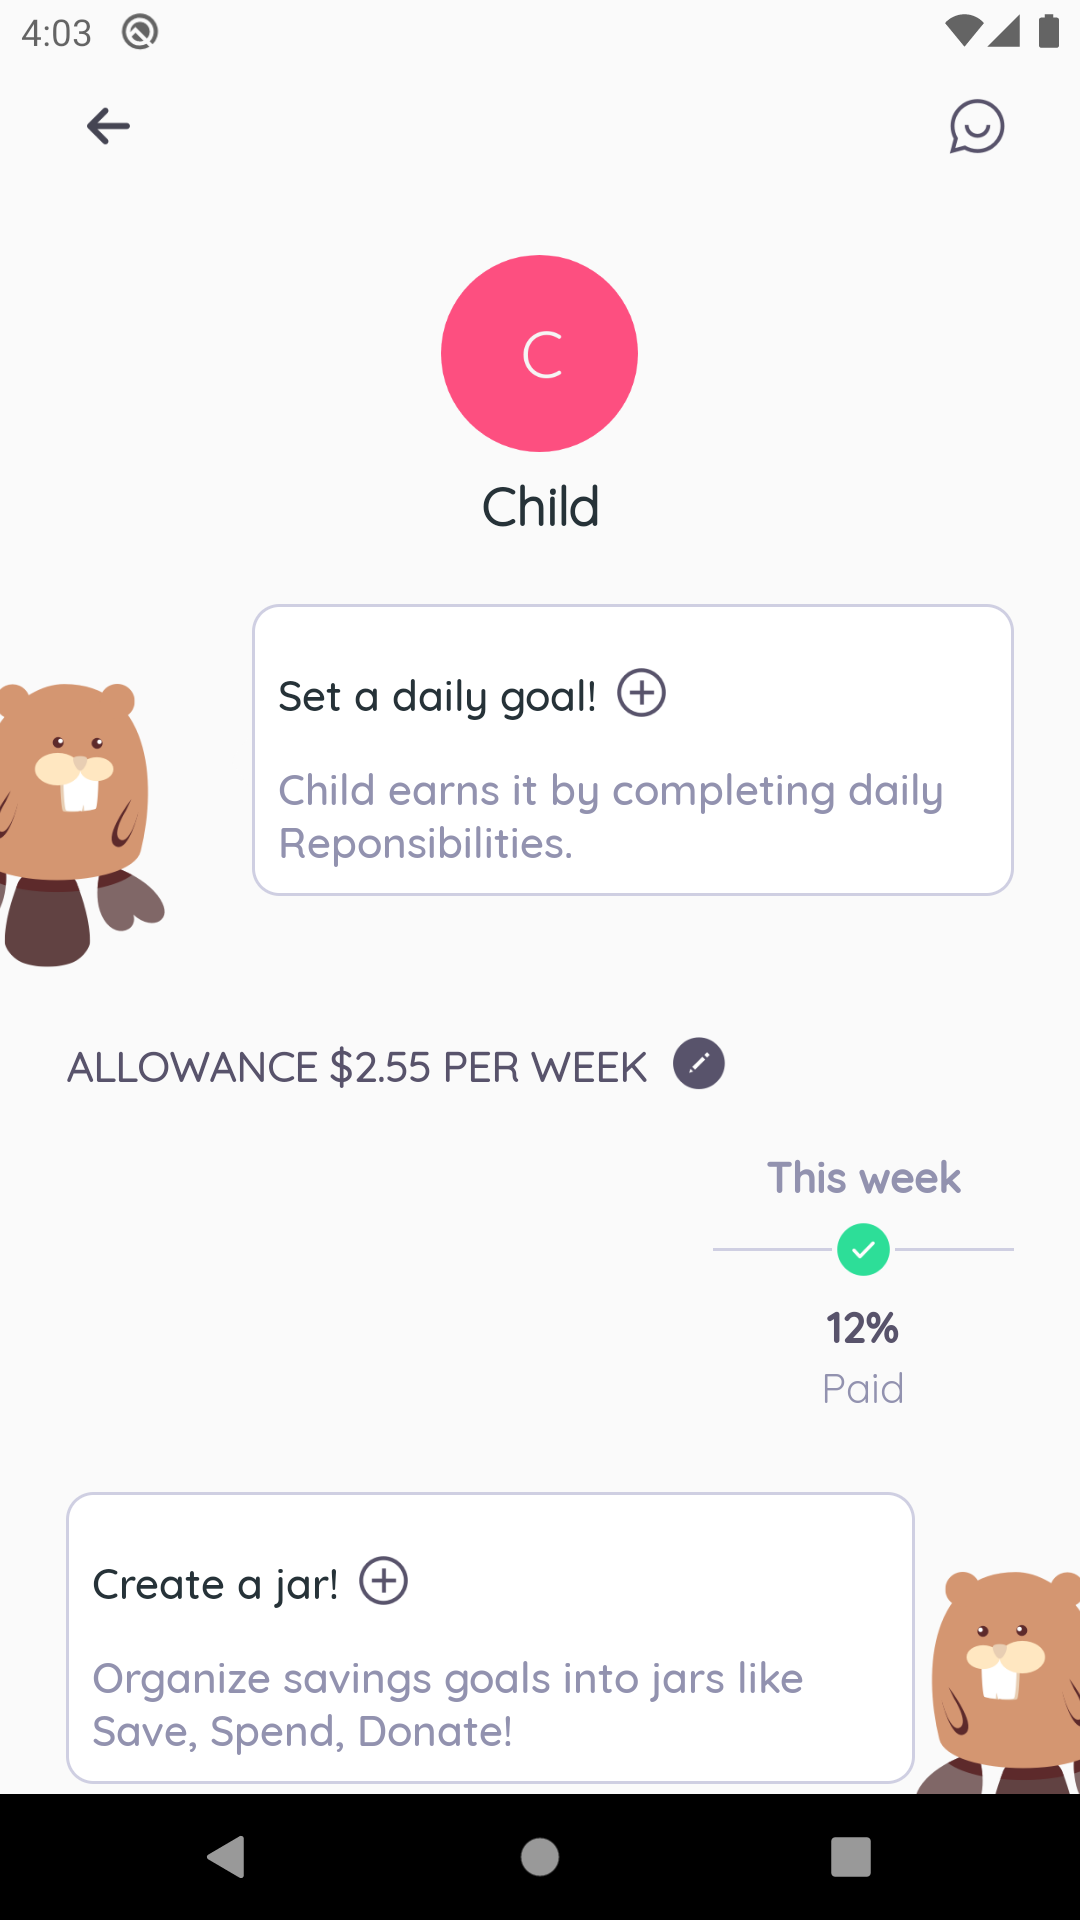
\includegraphics[width=.4\linewidth]{images/applications/Homey/Homey_3.png}} &
\subcaptionbox{Child's perspective}{ 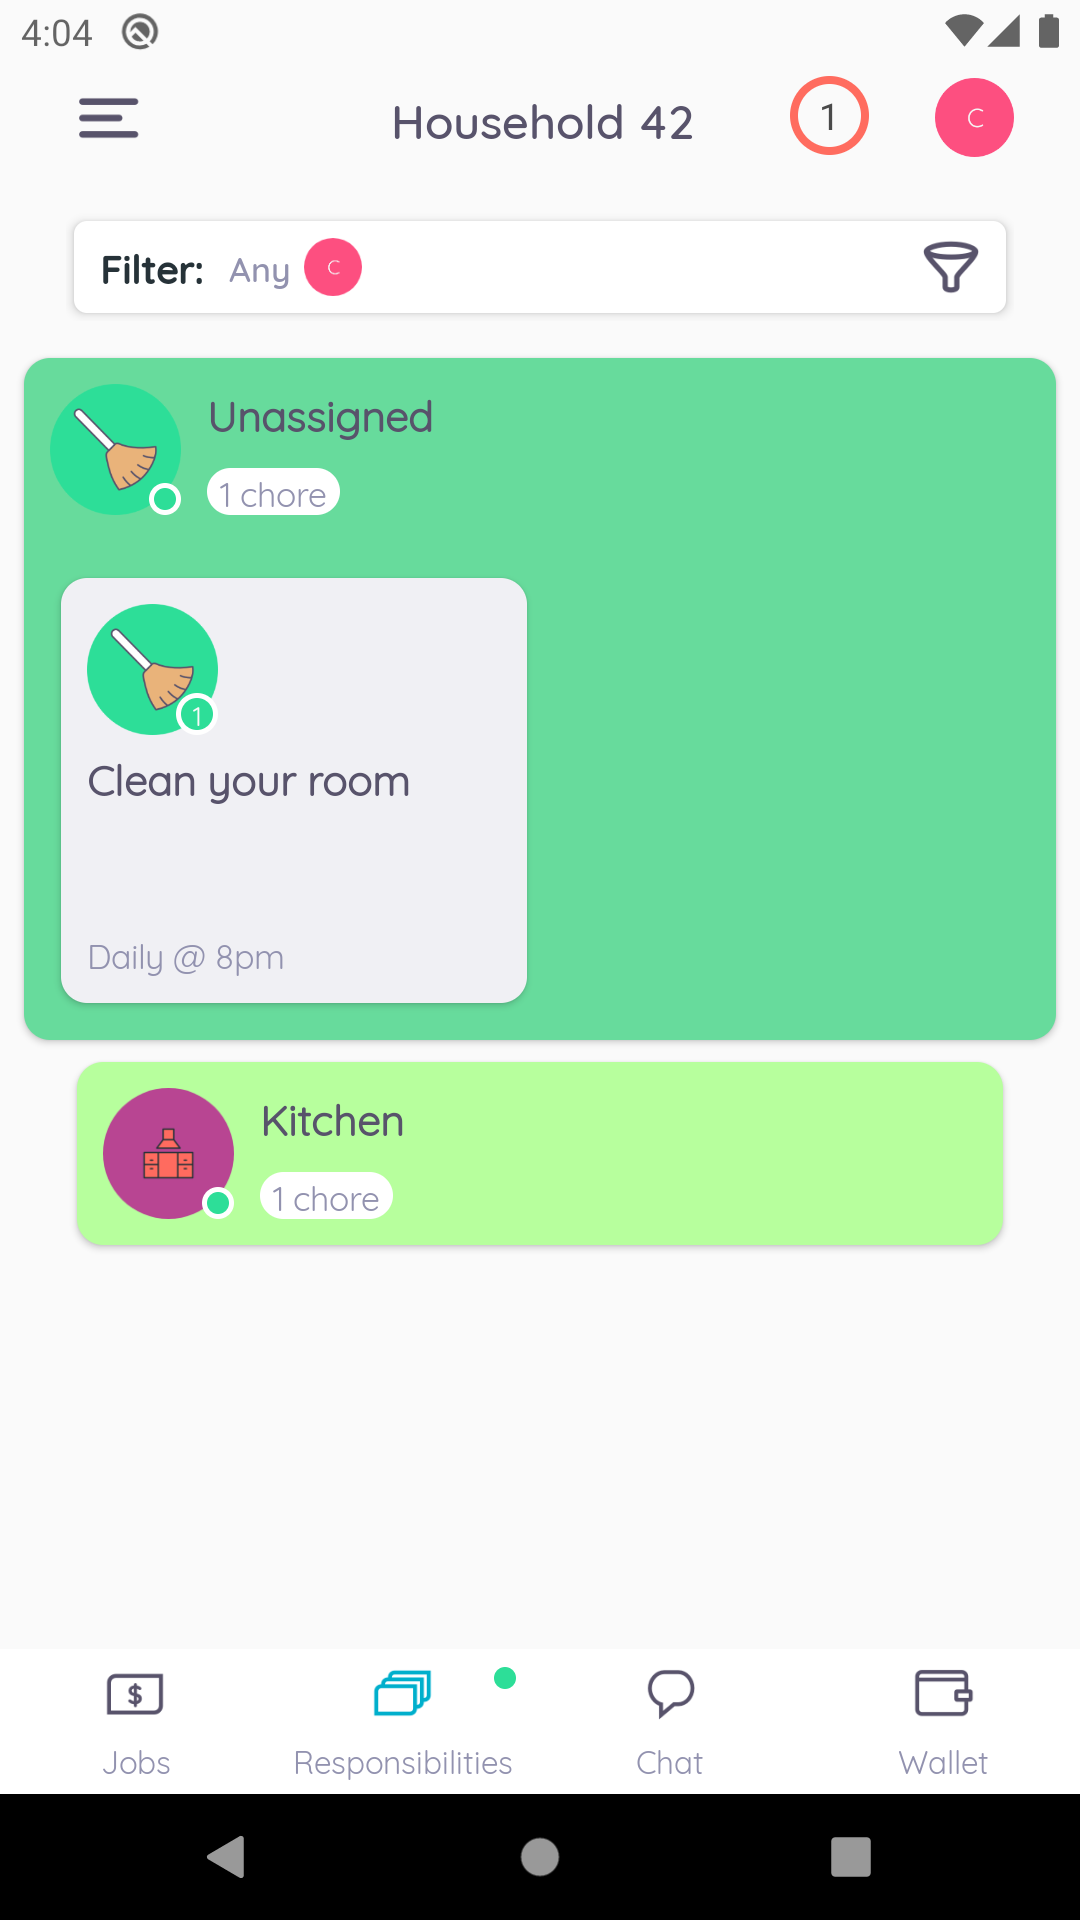
\includegraphics[width=.4\linewidth]{images/applications/Homey/Homey_4.png}}
\end{tabular}
\caption{\textit{Homey} application screenshots}
\label{fig:applications:homey}
\end{figure}

\begin{table}[htb]
\begin{tabularx}{\linewidth}{>{\parskip1ex}X@{\kern4\tabcolsep}>{\parskip1ex}X}
\toprule
\hfil\bfseries Advantages
&
\hfil\bfseries Disadvantages
\\
\cmidrule(r{3\tabcolsep}){1-1}\cmidrule(l{-\tabcolsep}){2-2}

Available on both platforms\par
Older Android versions support\par
Rich functionality

&

Low Google Play rating\par
Frequent crashes\par
Occasionally confusing design\par
Not many options in the free version

\\
\bottomrule
\end{tabularx}
\caption{\textit{Homey} application advantages and disadvantages}
\label{tab:applications:homey}
\end{table}

\subsection{S'moresUp}\label{subsec:market:solutions:smoresup}
\textit{S'moresUp} \cite{SmoresUpSmartChores,MoresUpBestChores} is an application that goes much beyond requirements. It is available on both Android and iOS platforms and is targeted to all age groups. It has more than 100000 downloads from Google Play and a rating of 4.0. The application requires at least version 4.4 of Android operating system and has a size of 19MB. Its last update was in October 2020.
\\\\
The application is intricate. It has many screens and options that tend to be overwhelming and illegible. Extra features like in-family social networking might lead to counterproductiveness. \textit{S'moresUp} tends to load data on every screen change, which causes severe delays interrupting the flow and slight issues with saving data. It has both parent's and child's perspective, however, requires a separate email account for every child. Despite free version providing more functionality than predecessors, only paid account allows usage without hindrance.
\\\\
Example screenshots of the \textit{S'moresUp} application were presented in Figure~\ref{fig:applications:smoresup}. A summary of its strengths and shortcomings was presented in Table~\ref{tab:applications:smoresup}.
\\
\begin{figure}
\centering
\begin{tabular}{cc}
\subcaptionbox{Family dashboard}{ 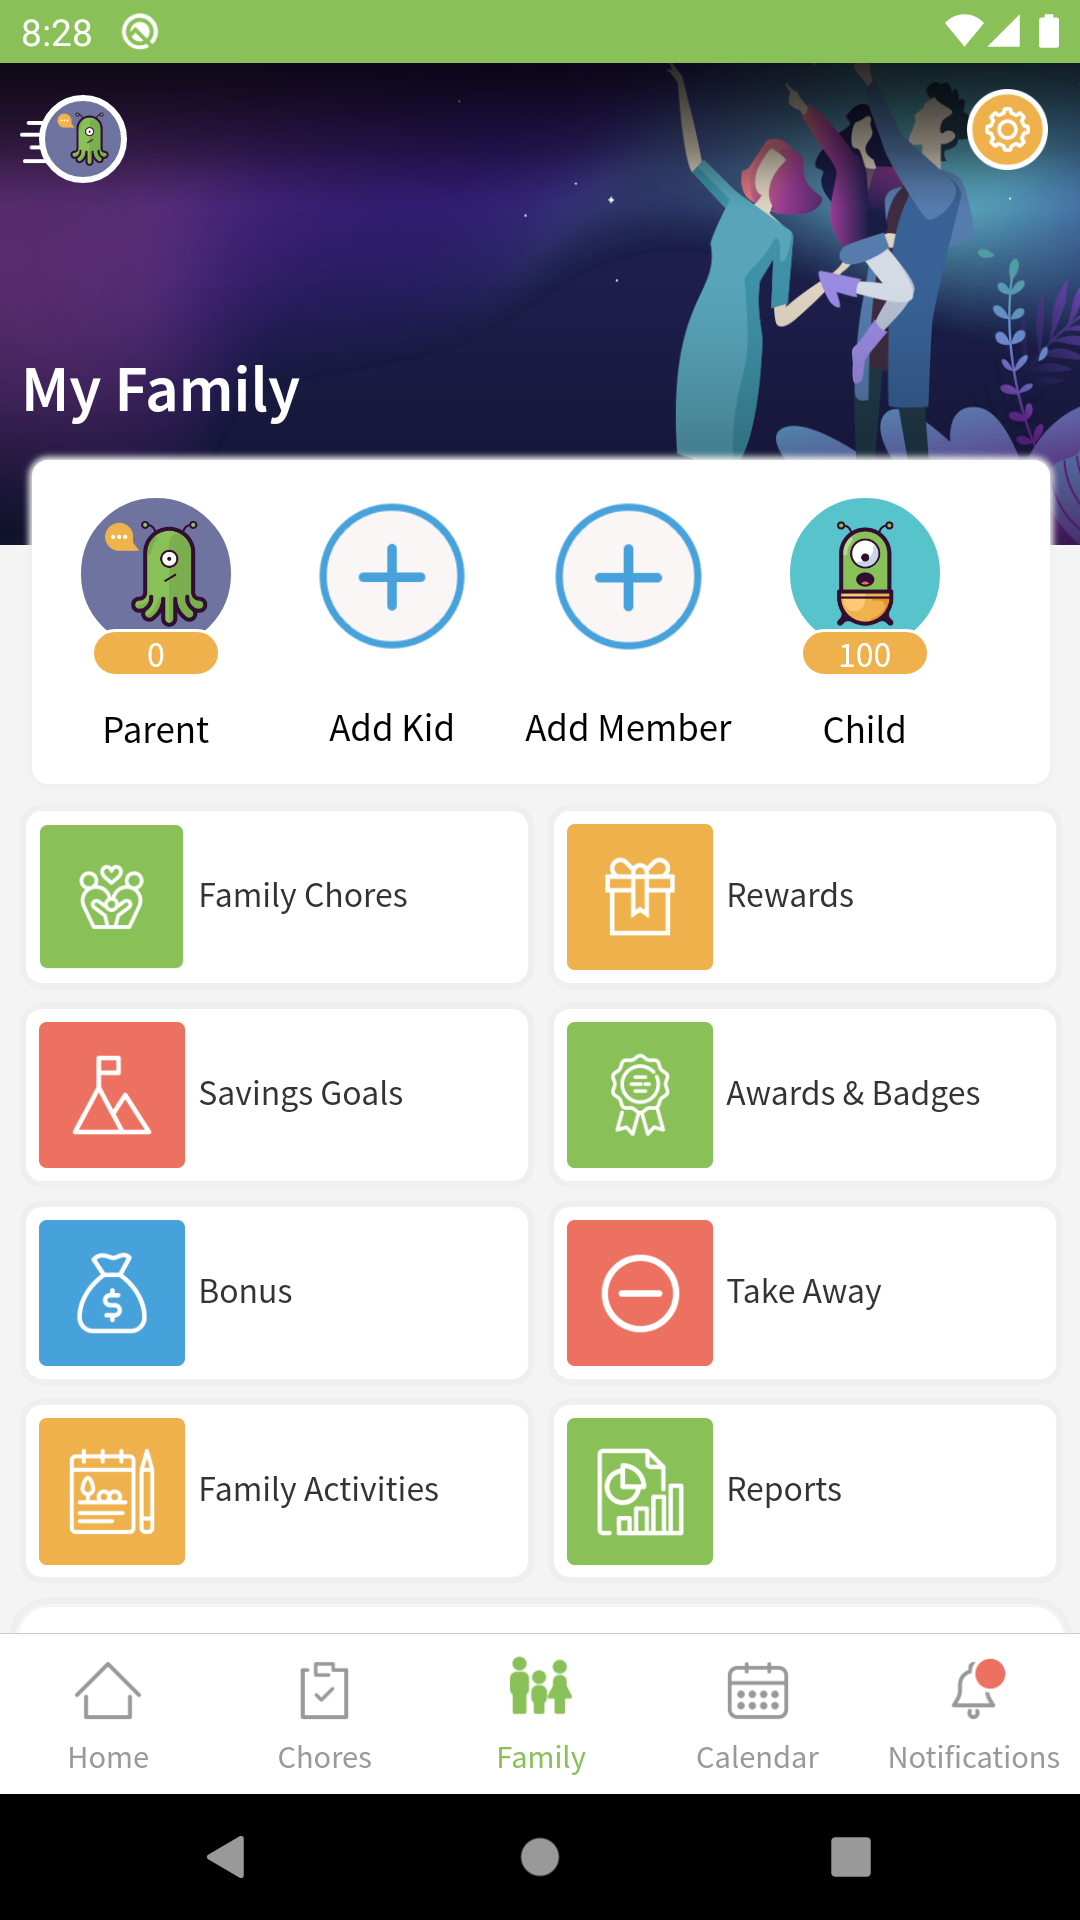
\includegraphics[width=.4\linewidth]{images/applications/SmoresUp/SmoresUp_1.png}} &
\subcaptionbox{Chores list}{ 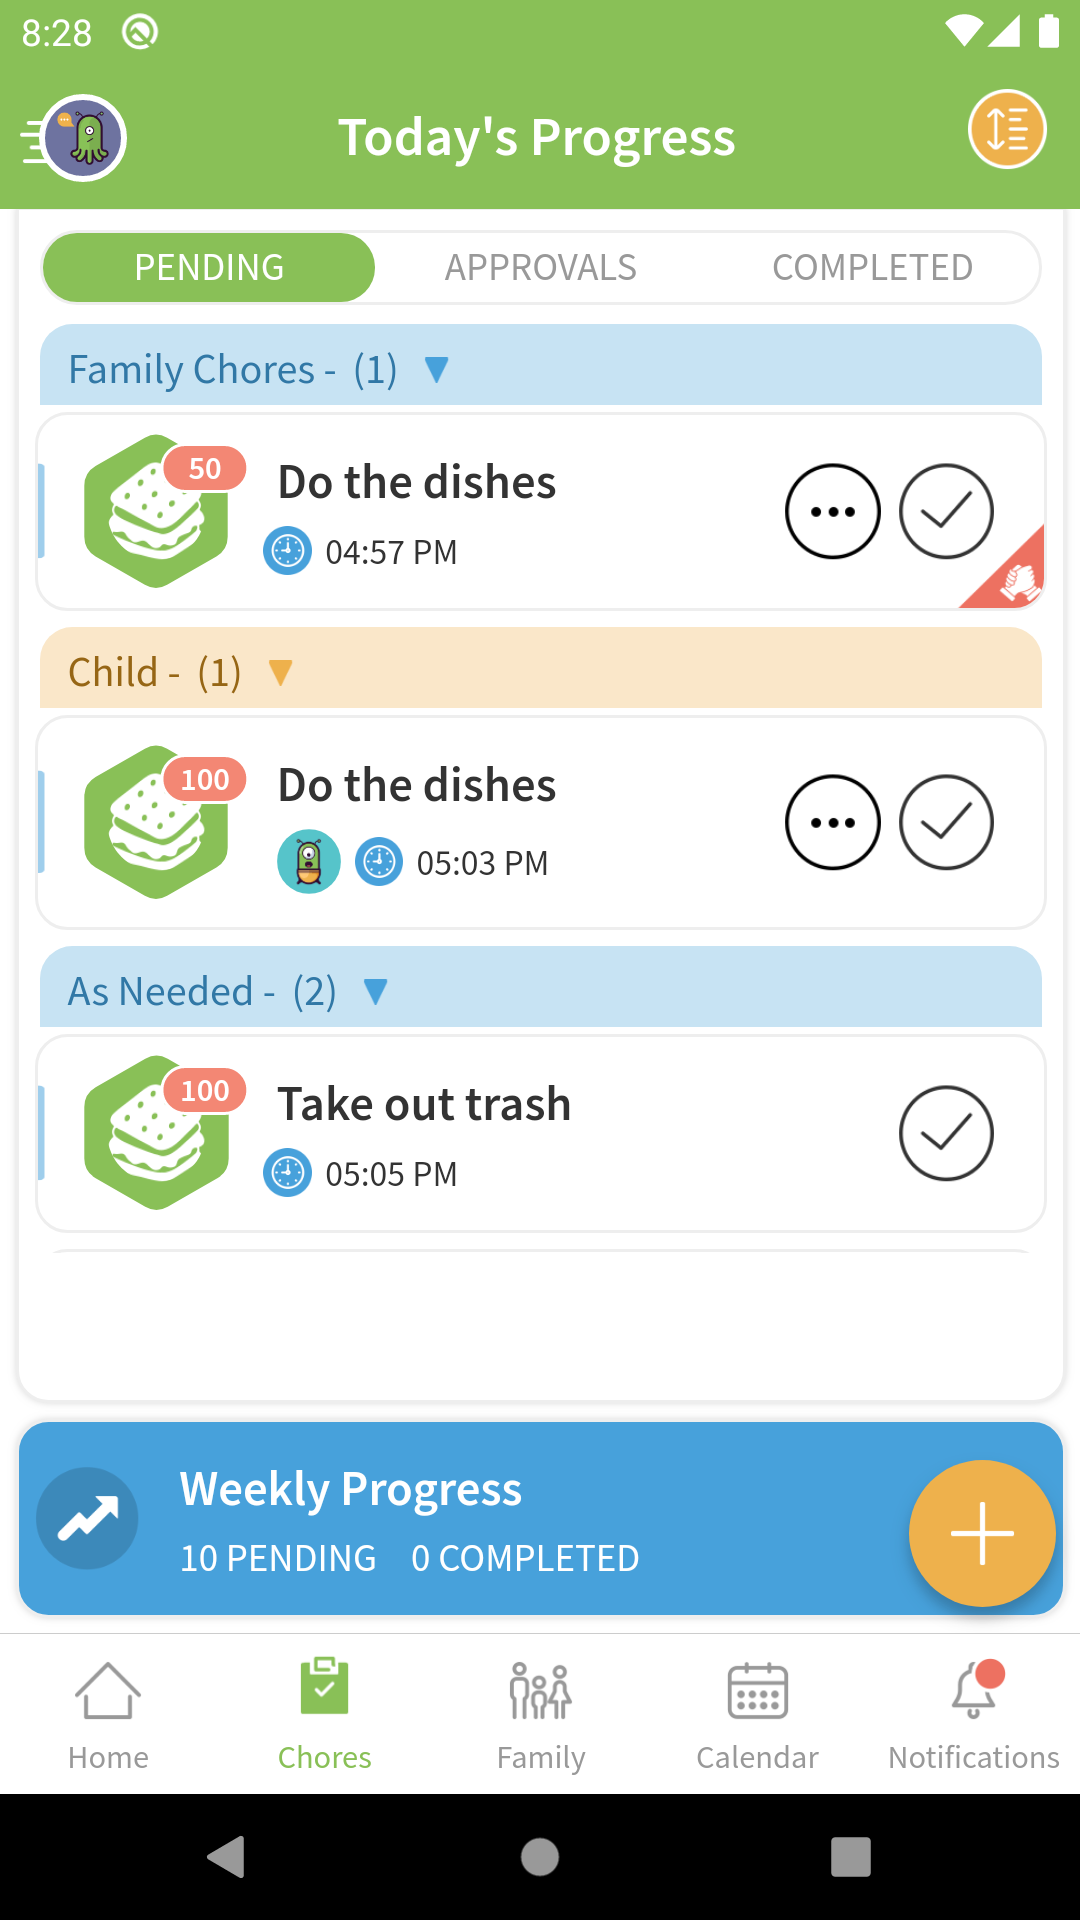
\includegraphics[width=.4\linewidth]{images/applications/SmoresUp/SmoresUp_2.png}} \\\\
\subcaptionbox{Social networking view}{ 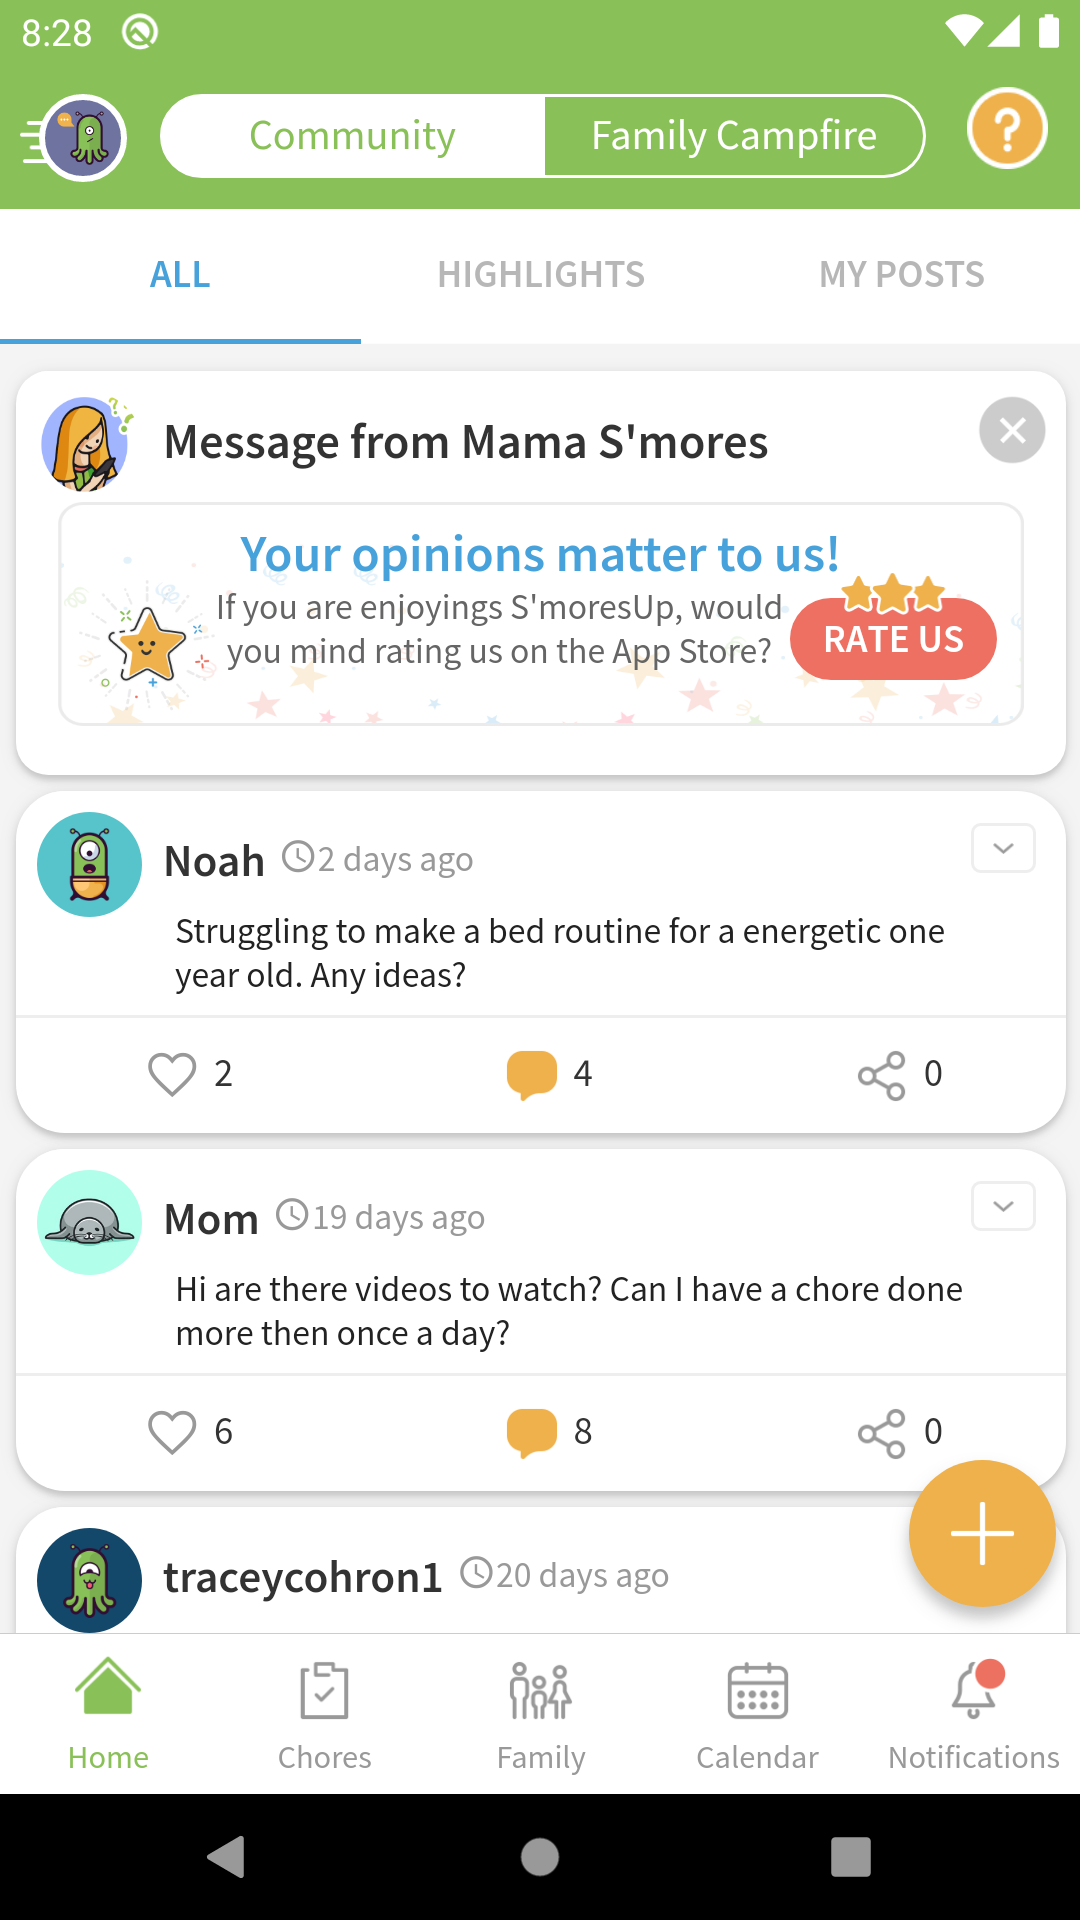
\includegraphics[width=.4\linewidth]{images/applications/SmoresUp/SmoresUp_3.png}} &
\subcaptionbox{Child's perspective}{ 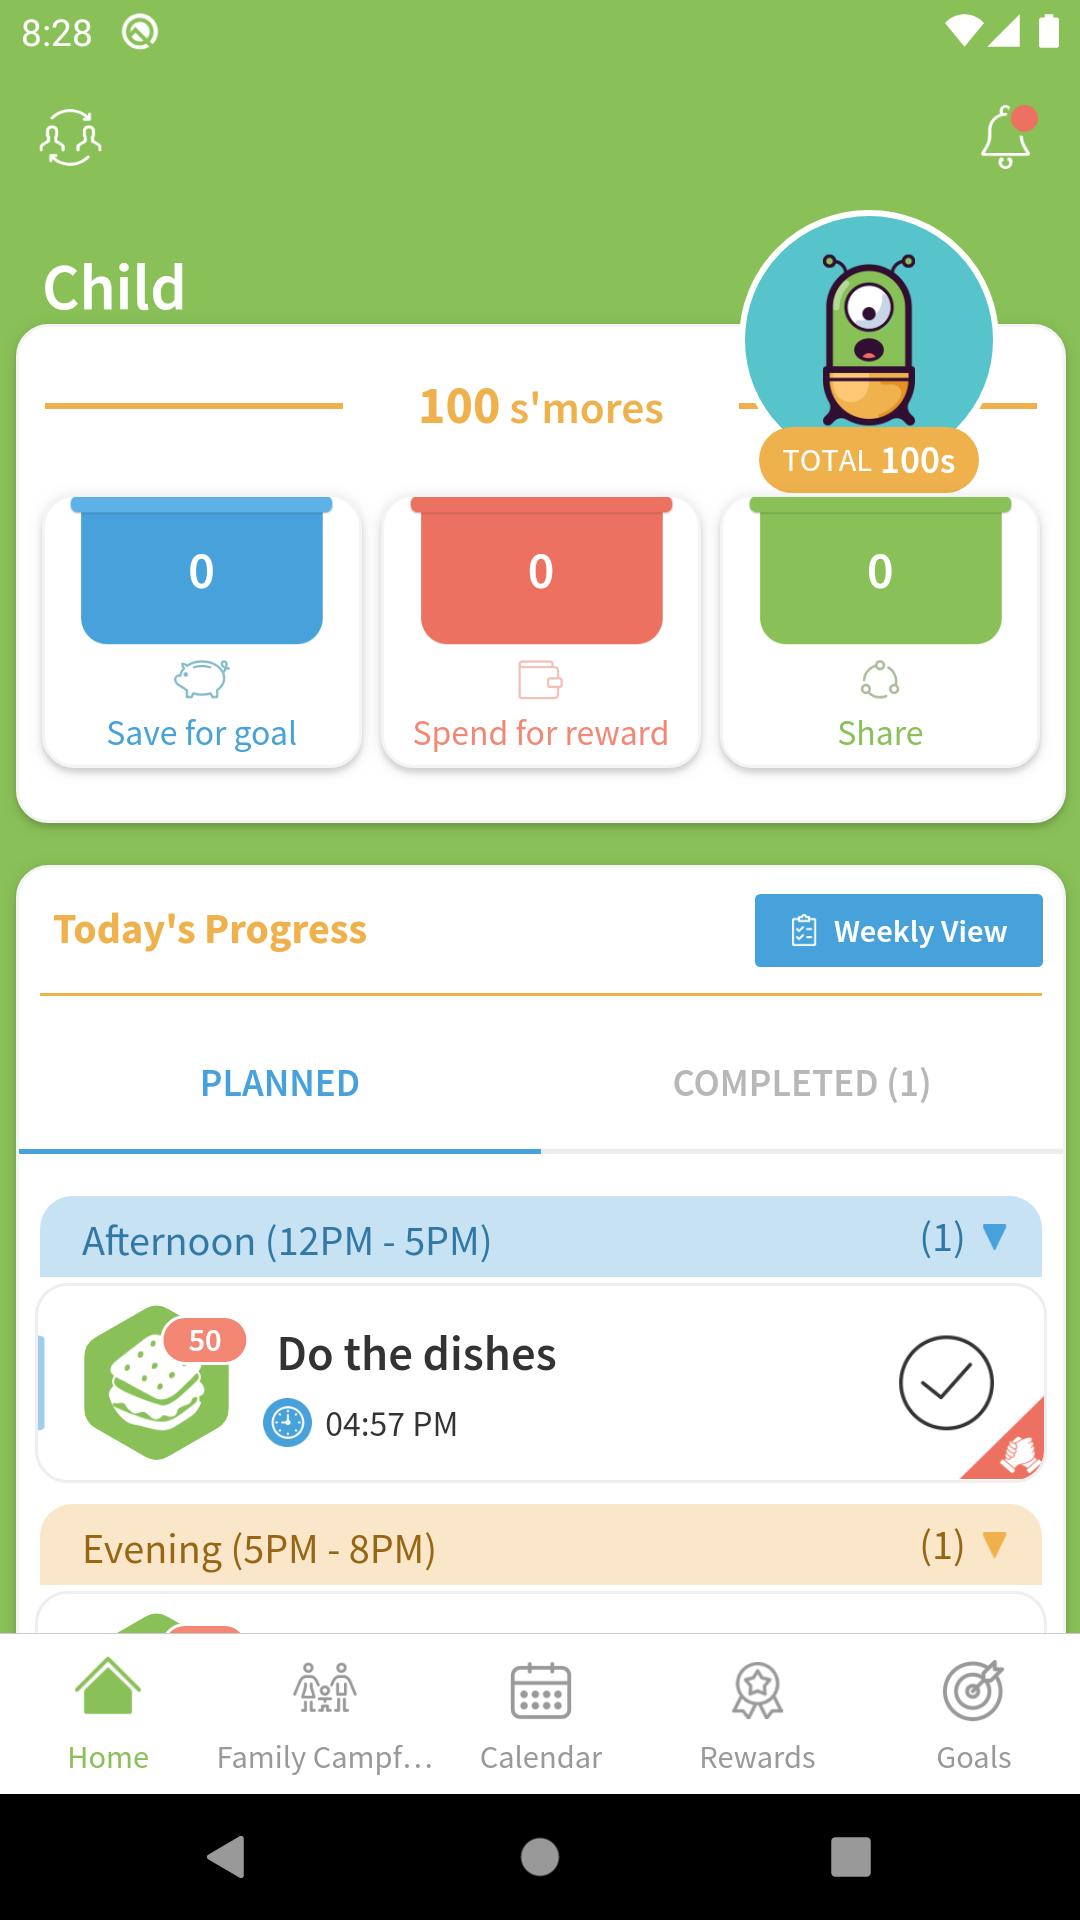
\includegraphics[width=.4\linewidth]{images/applications/SmoresUp/SmoresUp_4.png}}
\end{tabular}
\caption{\textit{S'moresUp} application screenshots}
\label{fig:applications:smoresup}
\end{figure}

\begin{table}[htb]
\begin{tabularx}{\linewidth}{>{\parskip1ex}X@{\kern4\tabcolsep}>{\parskip1ex}X}
\toprule
\hfil\bfseries Advantages
&
\hfil\bfseries Disadvantages
\\
\cmidrule(r{3\tabcolsep}){1-1}\cmidrule(l{-\tabcolsep}){2-2}

Available on both platforms\par
High Google Play rating\par
Small application size\par
Remarkably rich functionality\par
Abundant design\par

&

\par
Frequently confusing design\par
Counterproductive features\par
Long data load\par
Requiring email account for a child\par
Frequent purchase incentives

\\
\bottomrule
\end{tabularx}
\caption{\textit{S'moresUp} application advantages and disadvantages}
\label{tab:applications:smoresup}
\end{table}


\subsection{OurHome}\label{subsec:market:solutions:ourhome}
\textit{OurHome}\cite{OurHomeChoresRewards,OurHomeChoresRewardsa} serves the purpose of not only a productivity application but also a family organiser. It is available on both operating systems (Android and iOS) and targeted to everyone. With more than 500000 downloads it has a rating of 3.6. It requires Android in version 5.0 or higher. Its size is 6.7MB, and the last update was in October 2020.
\\\\
\textit{OurHome}'s design is very tidy, but one might find it slightly confusing nonetheless. Instead of separate child's and parent's perspective, it offers an \textit{admin} account, but it does not seem to function as intended. It has features going beyond the core features defined in the Project Assumptions chapter (\ref{sec:assumptions:features}), such as a calendar or grocery list, as well as many pre-defined tasks. All of the features are free. Data load times occasionally are longer than expected.
\\\\
Example screenshots of the \textit{OurHome} application were presented in Figure~\ref{fig:applications:ourhome} - Rewards list screen was captured during excessive load time. A summary of its benefits and drawbacks was presented in Table~\ref{tab:applications:ourhome}.
\\
\begin{figure}
\centering
\begin{tabular}{cc}
\subcaptionbox{Family view}{ 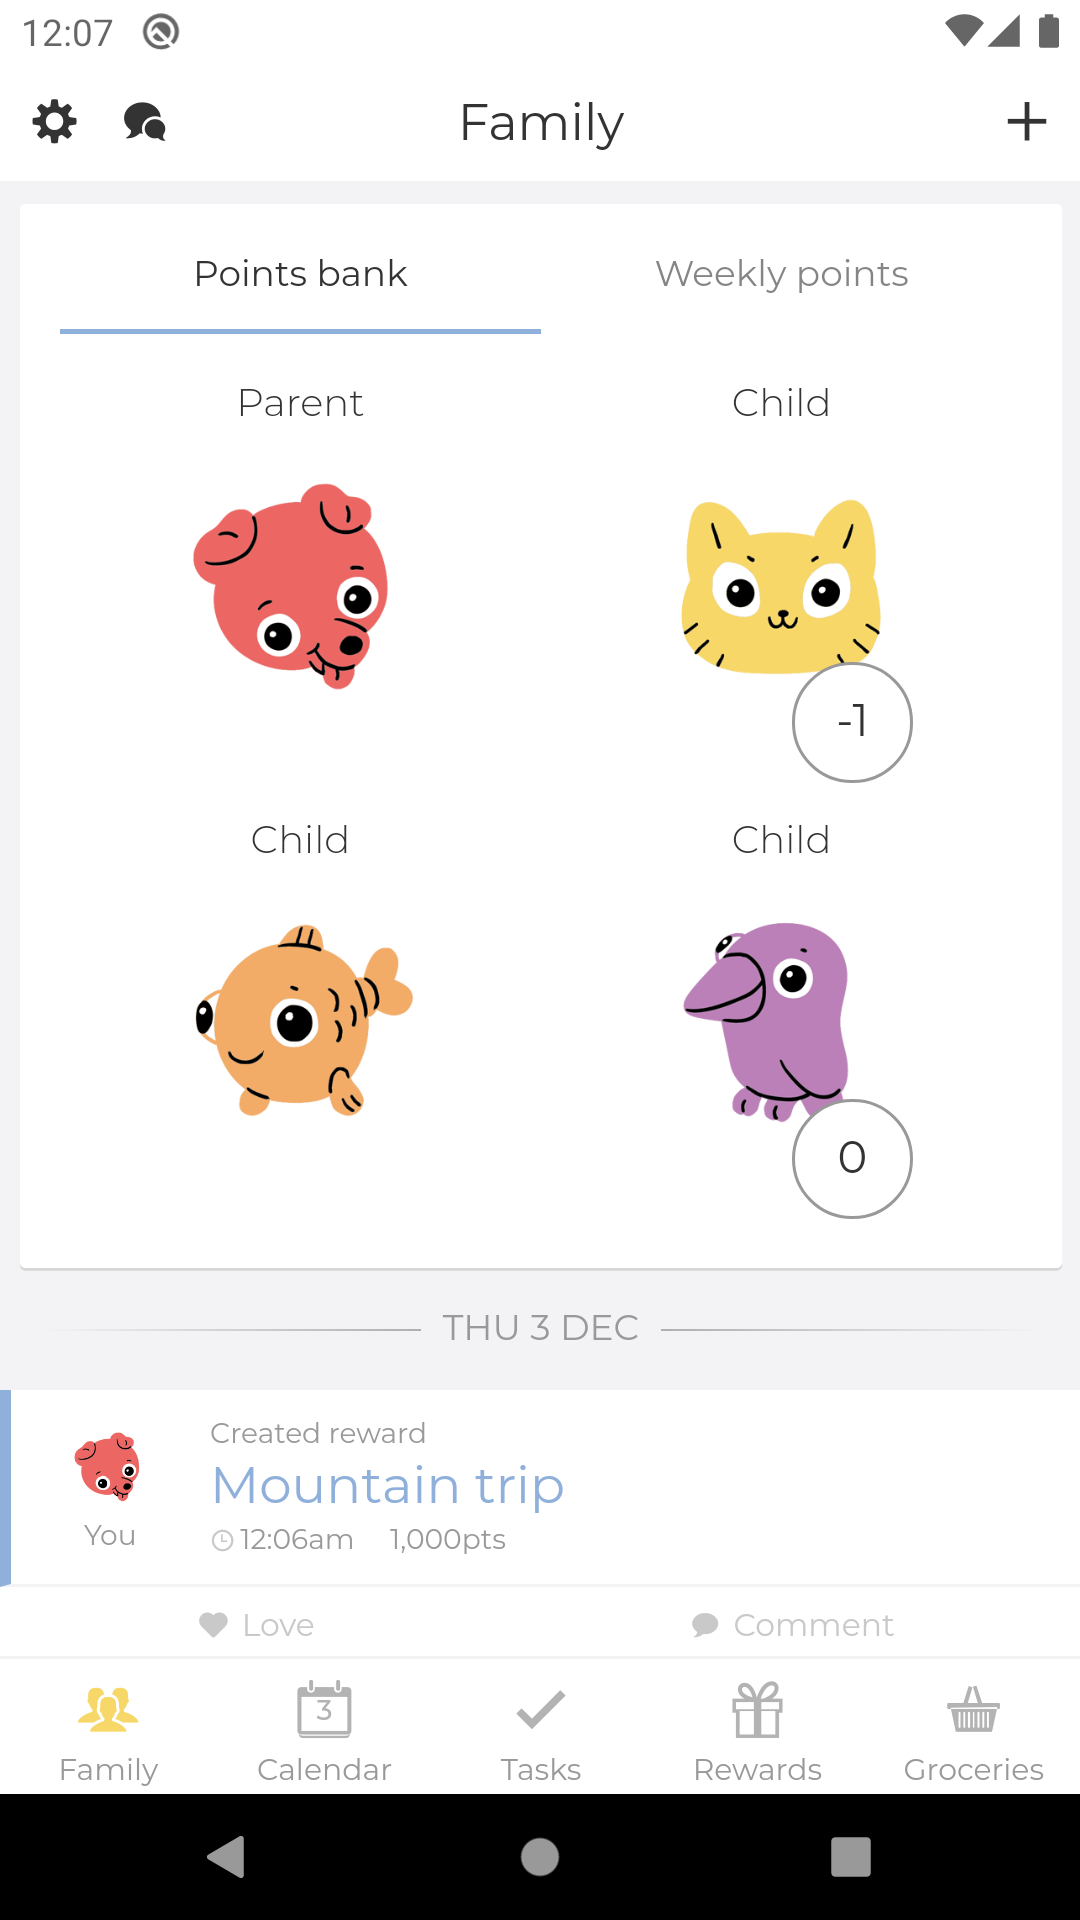
\includegraphics[width=.4\linewidth]{images/applications/OurHome/OurHome_1.png}} &
\subcaptionbox{Tasks list}{ 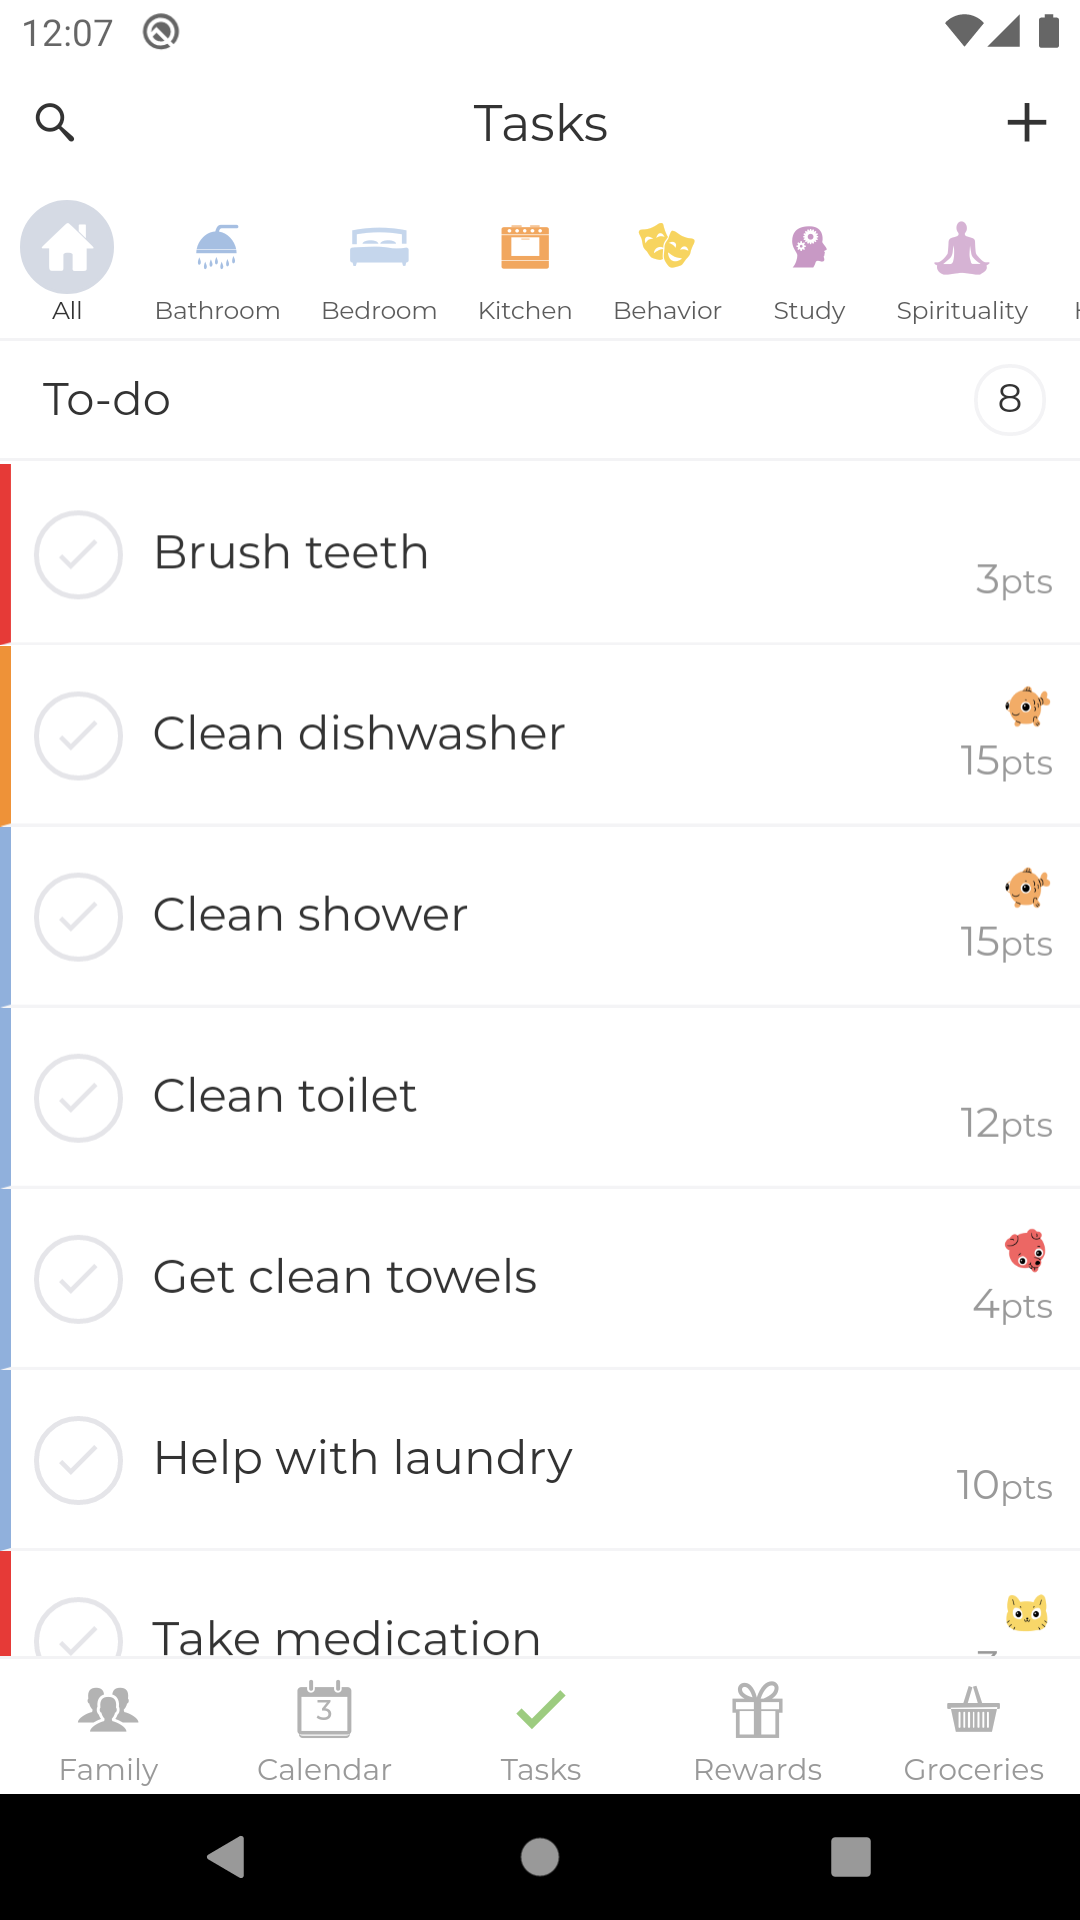
\includegraphics[width=.4\linewidth]{images/applications/OurHome/OurHome_2.png}} \\\\
\subcaptionbox{Rewards list}{ 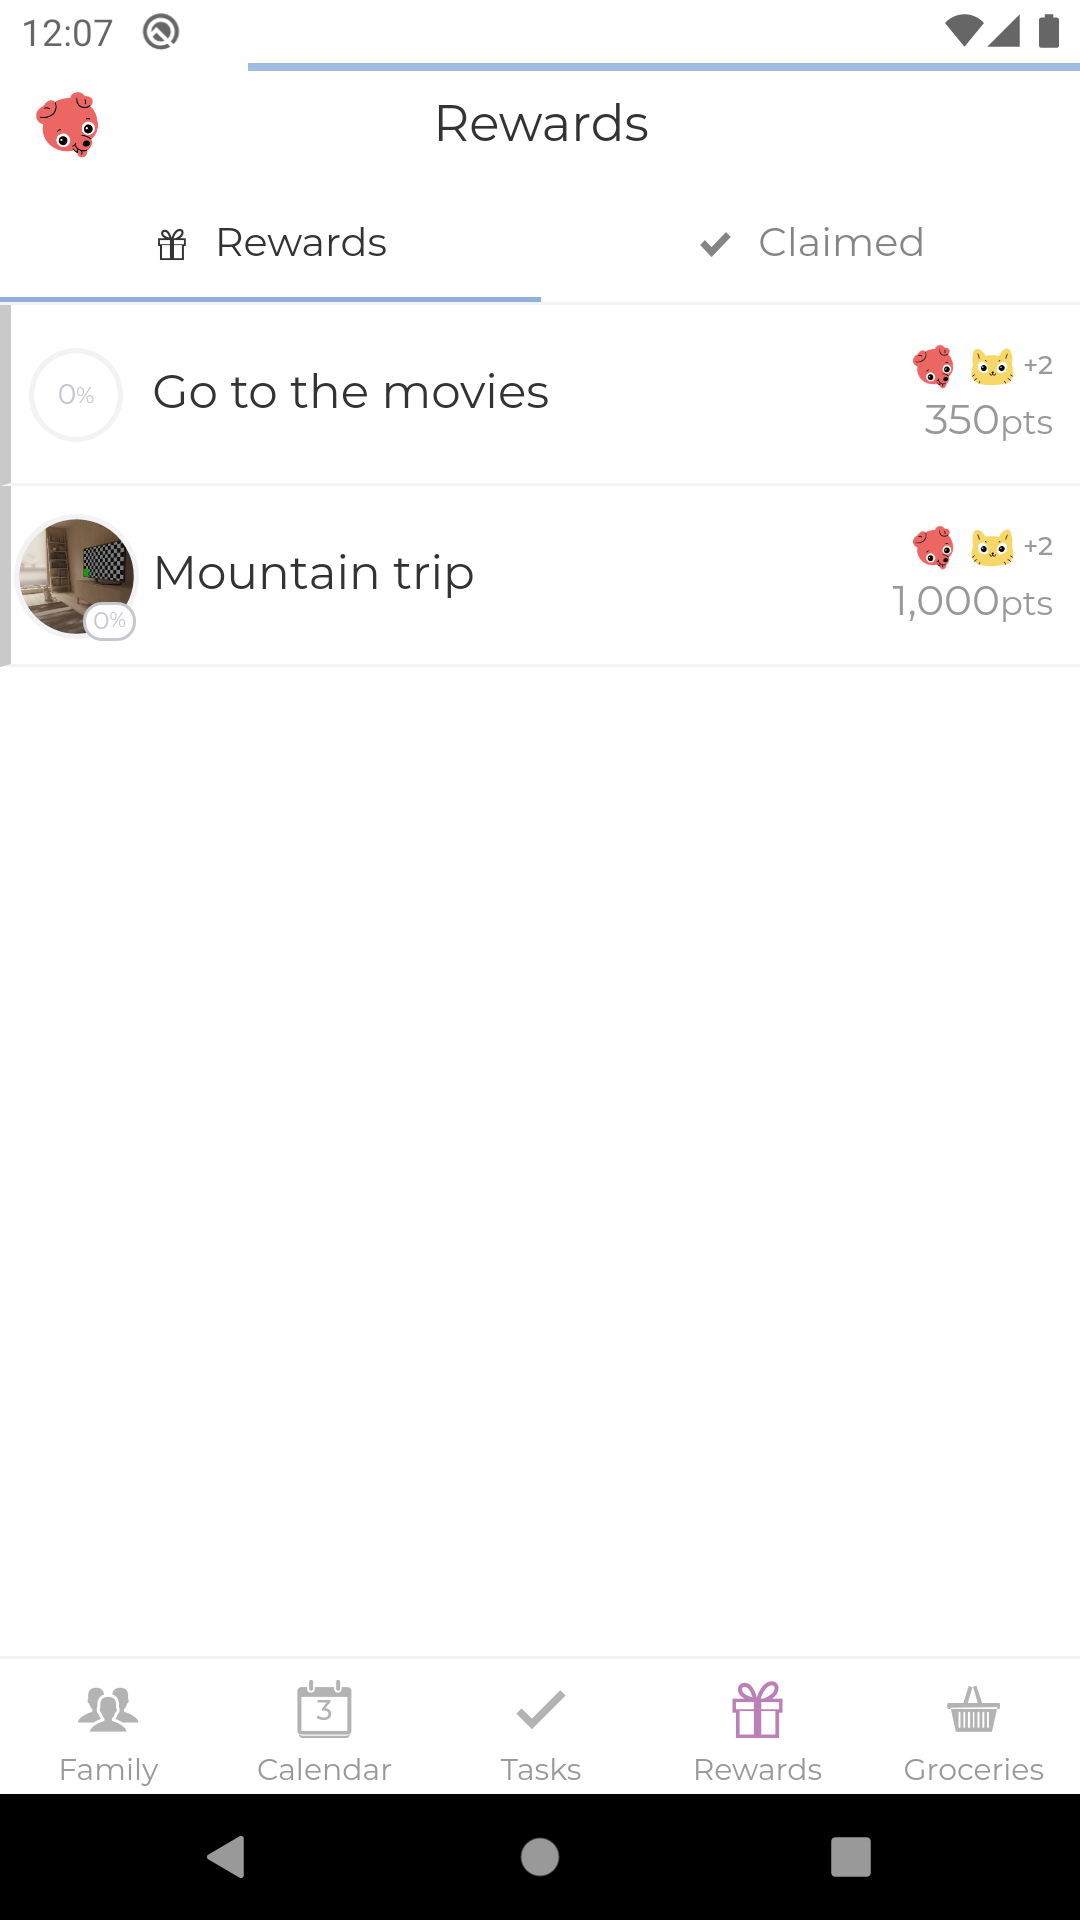
\includegraphics[width=.4\linewidth]{images/applications/OurHome/OurHome_3.png}} &
\subcaptionbox{Groceries list}{ 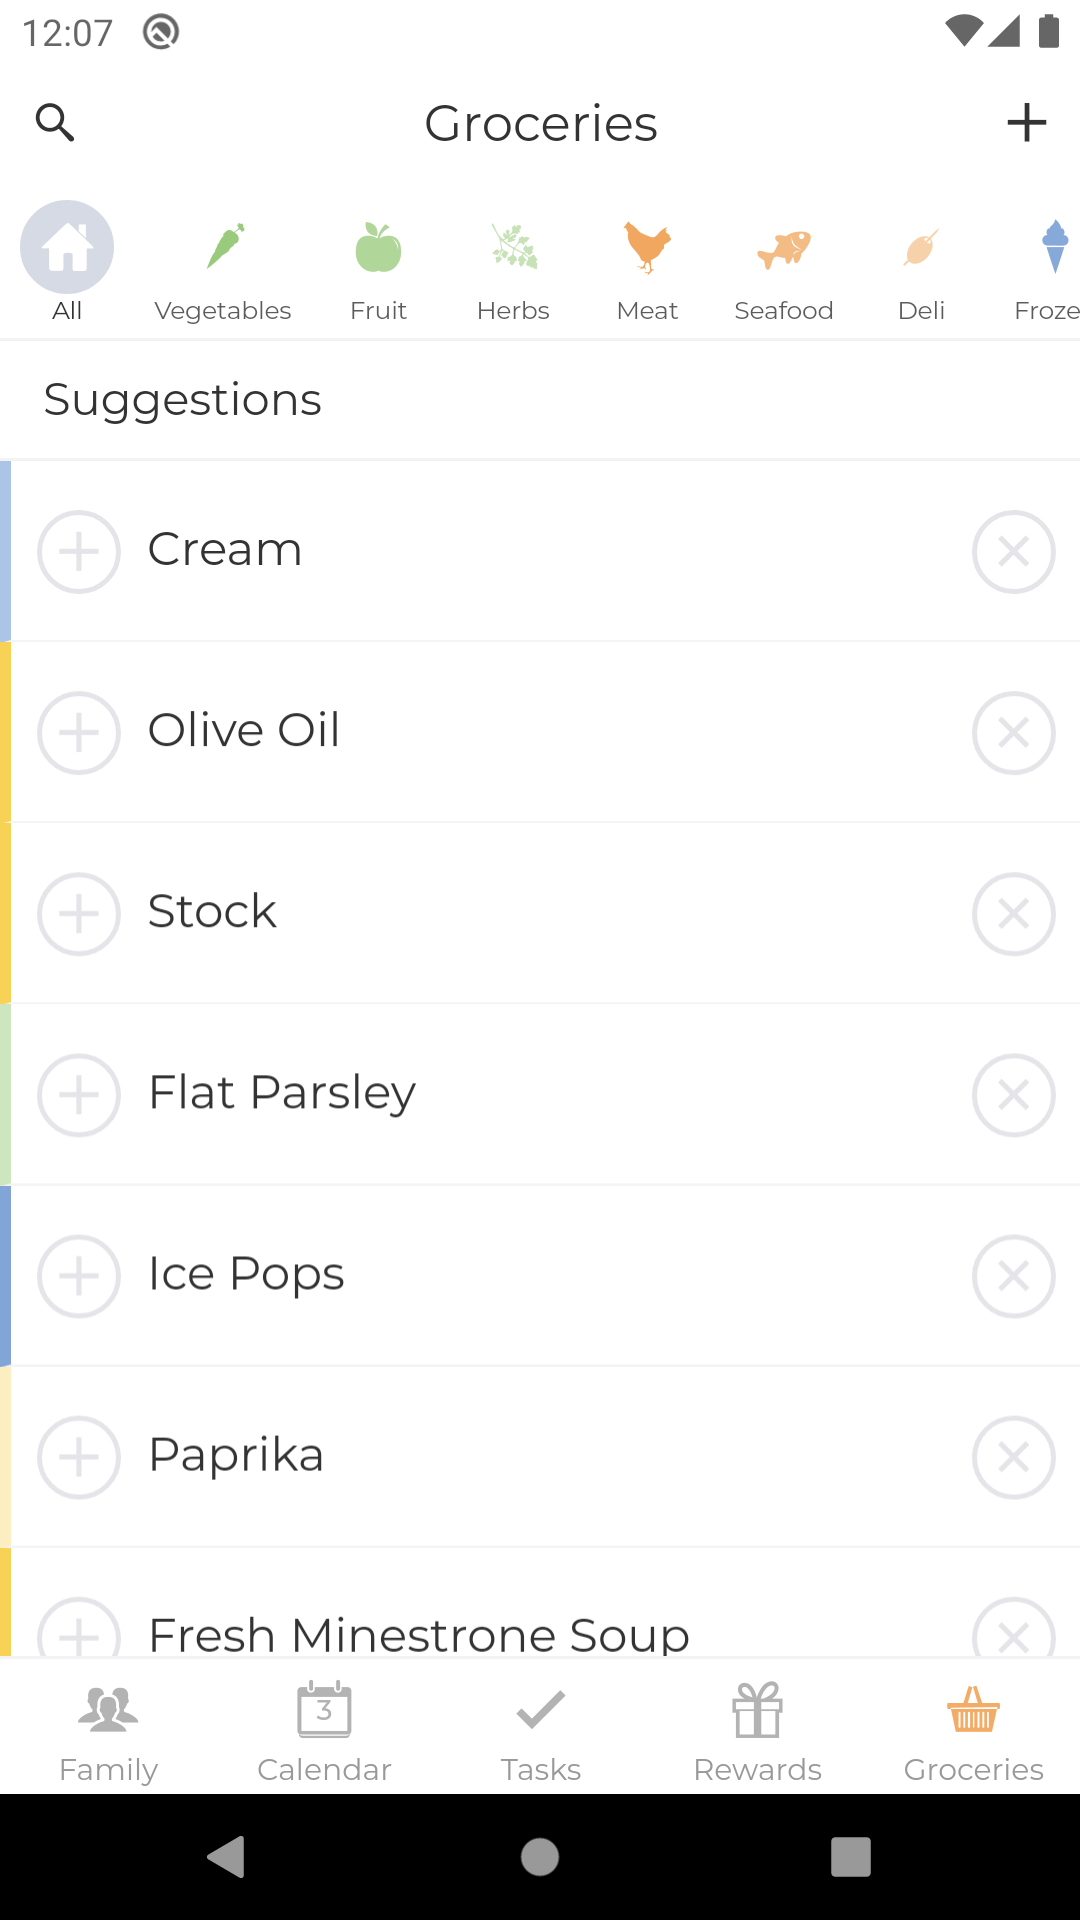
\includegraphics[width=.4\linewidth]{images/applications/OurHome/OurHome_4.png}}
\end{tabular}
\caption{\textit{OurHome} application screenshots}
\label{fig:applications:ourhome}
\end{figure}

\begin{table}[htb]
\begin{tabularx}{\linewidth}{>{\parskip1ex}X@{\kern4\tabcolsep}>{\parskip1ex}X}
\toprule
\hfil\bfseries Advantages
&
\hfil\bfseries Disadvantages
\\
\cmidrule(r{3\tabcolsep}){1-1}\cmidrule(l{-\tabcolsep}){2-2}

Available on both platforms\par
Small application size\par
Rich, free functionality\par
Tidy design\par

&

\par
Occasionally confusing design\par
Non-functional child's perspective\par
Infrequent long data loads

\\
\bottomrule
\end{tabularx}
\caption{\textit{OurHome} application advantages and disadvantages}
\label{tab:applications:ourhome}
\end{table}


\section{Conclusions}\label{sec:market:conclusions}
It is crucial to draw conclusions from the competition analysis. There are several categories of opportunities and obstacles that are especially important:
\begin{itemize}
\item Design and user experience
\item Functionality
\item Performance
\end{itemize}

\subsection{Design and user experience}\label{subsec:market:conclusions:design}
One of the most distinctive issues all of the applications face is design and user experience. The layout is either not engaging enough or perplexing. It ought to be tidy, child-friendly and simple in order to minimise the risk of user loss. Several analyzed applications rely on \textit{Material Design} \cite{MaterialDesign} design system, which helps to provide clear interface but, if not used correctly or abused, might lead to confusion or a raw, unappealing design.

\subsection{Functionality}\label{subsec:market:conclusions:functionality}
Functionality, even if extensive, should always serve the primary purpose of the application. Derogations like social networking in \textit{S'moresUp}, while attractive business-wise, could not be implemented in the project. Thoroughly polished features are of at least the same importance. \textit{Quality over quantity} should apply to the final product's functionality.


\subsection{Performance}\label{subsec:market:conclusions:performance}
Even intermittent application crashes or lags might cause a tremendous user loss. It is a case of \textit{Homey - Chores and Allowance} and \textit{OurHome} and is reflected in user ratings and reviews. The implemented application should be stable and working smoothly, without long waiting times.